\section{Industry \& Metropolitan Police Investigators} 
In order to gain feedback from the target end-users of this tool I arranged a meeting with Mat Stanley, a Detective Sergeant of a London Metropolitan Police crypto-currency investigation unit and, in order to also gain a private sector industry perspective, Iggy Azad who is a senior investigator at Coinbase. Iggy Azad was previously also with the Metropolitan Police before taking on a private sector role at Coinbase. 
\\\\
I arranged the meeting with the goal of obtaining critical feedback on the investigation tool based on their domain knowledge of carrying out investigations and their experience with other similar proprietary tools which have been built to achieve similar goals. I also wanted to better understand the challenges that law enforcement face when investigating crypto-currency based crime and potentially what the current solutions are not adequately providing the investigators with. 

\subsection{Successes and Weaknesses}
Through my conversation with Mat and Iggy, and through demonstrating the current functionality of the tool, I obtained feedback such that I was able to identify areas of success and areas of weakness in the current implementation. These areas are summarised below:

\begin{itemize}
    \item \textbf{Weakness}: The different types of nodes aren't very clear (\textit{Implicit: I had to explain what the different types of nodes represent}). \textbf{Actionable}: Introduce UI feature to make the types of nodes more apparent. 
    \item \textbf{Success}: The date and price filtering functionality is often very valuable to investigators. This is often particularly useful when tracing funds through a mixing service [see \ref{background-mixing-service}]. 
    \item \textbf{Success}: Displaying the historical exchange rate is also very important to investigators; this enables them to better understand the true value of the flow of funds, which may be otherwise difficult without historical exchange rates due to the volatility in the value of Bitcoin. 
    \item \textbf{Success \& Weakness}: The Path Finding feature is very useful in investigations, yet not provided by some of the solutions they currently use. However, It would be useful to be able to type the name of a wallet rather than an address and the path finding happen for any address belonging to the wallet. 
    \item \textbf{Success}: Clustering using the wallet information obtained in section \ref{section-entity-tagging} will prove extremely useful; this data is also provided by their ChainAnalysis software. 
    \item \textbf{Success}: The ability to toggle on/off clustering heuristics is very desirable and not provided by several other solutions. 
    \item \textbf{Success \& Weakness}: Ability to add custom information (through the custom node feature) is very useful; however, adding information such as Photographic ID is not usually required at this stage of the investigation. The tool will be used in the run up to issuing a warrant to obtain identification from exchanges (who should have it due to KYC [see Know Your Customer \ref{background-kyc}). Additionally, adding this additional data would be more intuitive to exist as data associated with a node, rather than existing as a separate node itself. 
    \item \textbf{Weakness}: Secure data storage not addressed by current deployment : If storing investigation specific data, a secure solution is needed such that only the user could access it. 
\end{itemize}

\subsection{Current Solutions}
Mat spoke about the current solutions employed at the Met Police in order to help investigate crimes; these solutions include proprietary software, such as ChainAnalysis, and several others as described in section \ref{background-existing-tools}. 
\\\\
Questioned why so many tools were used, Mat explained that each tool provides something different, such as different clustering heuristics or their data has originated from a different source. Often data obtained from each tool is distinct, but complementary to the overall investigation.  

\subsection{Desirable features}
There were a number of features Mat and Iggy explained are very useful to their investigations and are often provided by the current solutions that they use, but were not provided by my tool. These are:
\begin{itemize}
    \item Support for several crypto-currencies. Namely: Ethereum, Litecoin, Bitcoin, Bitcoin Cash, Dash
    \item Ability to save a graph state as an investigation and come back to it later
    \item Ability to export the data from an investigation, often in CSV format to provide evidence for cases - needs to be digestible by a jury.
    \item Ability to set up notifications/watches for state changes on entities - e.g an address/wallet receives or spends funds 
    \item Automatically detect and alert when an address re-surfaces in a new investigation that was seen in a previous investigation 
    \item Ability to collapse nodes/remove nodes from graph 
    \item Offering a compliance/risk score with clustering information - is the data verified? Does the data come from multiple independent sources? 
    \item Enhance clustering of addresses by considering different types of addresses [see address types \ref{background-address-types}]
    \item Incorporate address tag information - they often have some significance, e.g tags may relate to a gamer tag which can be searched for in other datasets. Also vanity addresses often have significance, may include parts of their name which can be used to help link addresses [see vanity addresses \ref{background-vanity-addresses}]
\end{itemize}

\subsection{Data Sources}
In addition to the additional features, Mat and Iggy also helped me additional types of resources that can be used as datasources to feed functionality for the tool. These data sources are:
\begin{itemize}
    \item oxt.me : Useful for looking at multi-signature transactions
    \item bitcoinswhoswho.com : Check addresses against reported scams or see if the address has associated tags
    \item Shapeshifter : Given a TXID, tells you where the coin went (which currency?). Also has a free API! Could integrate this information into the tool to help track funds across crypto-currencies. 
\end{itemize}

Furthermore, regarding beginning an investigation, Mat and Iggy spoke about how addresses of interest may be discovered to use as a starting point of an investigation:
\begin{itemize}
    \item Donation Requests: For example Wiki Leaks or Greenpeace donation addresses. 
    \item Bitcoin addresses that have been found on machines seized as part of an investigation. 
    \item Addresses in chat-rooms (e.g telegram) or on forum sites such as Reddit
\end{itemize}

\subsection{Future of Crypto-Currency Law Enforcement}
The uptake of crypto-currencies with even stronger privacy-preserving features is a cause for concern to law enforcement; crypto-currencies such as Monero [see \ref{background-monero}] make many currency investigation techniques unsuitable for investigating criminal activity using Monoero. Mat stated this is an issue, however due to the sophistication of Monero and its relative difficulty of use, such a low proportion of criminals are understood to be using it, in comparison to Bitcoin usage. There is additionally hurdles in the way of users wishing to buy and sell Monero; Mat referred to an example where, in Japan, exchanges will have their license remove if they accept Monero.

\section{Performance} 
\subsection{Individual Cypher Query Profiling}
In this section, I use the Cypher command \texttt{PROFILE} to profile queries in isolation for randomly selected data. Note that queries are profiled in isolation, with no other load on the database when they are executed. 
\\\\
Through profiling, it became clear that Neo4J would cache recently executed query search results, and therefore repeating the same query would have a significantly reduced response time. 

\subsubsection{Selecting random ID's to query}
In order to prevent the Neo4J instance from performing some caching on the address, the database must have not seen the address in a query before. Therefore, to retrieve the addresses to use in the profiled commands, I used another instance of Neo4J on my local machine to collect the ID's to use. This will help better reflect the performance of the queries that will be executed for the users address searches when a cache hit will be highly unlikely. I executed the following query to retrieve the addresses to use: \texttt{MATCH(n:ADDRESS) RETURN n LIMIT 20} where 20 is how many ID's i would like to profile. 

\subsubsection{Results}

With the 20 ID's, I then profiled each of their MATCH queries with the query:
\texttt{PROFILE MATCH(n: ADDRESS {address:'...'}) RETURN n}

\begin{center}
\begin{tabular}{ |c|c| } 
 \hline
\textbf{address} & \textbf{response time} \\\hline
14KTLEerB7uWPYZ5KcsxrJZwhFUDVwX9ZN & 22ms \\ 
14NHfjeRs7vPFVKkAhQg8hWbFr1cemtP1X & 17ms \\ 
14NNcfY2eFjG5YCC2DmgZfjj8kYmfAvWNs & 151ms \\ 
14NvmcsMQsMmmWkjYQz4XWKFYFZVvjtwg1 & 16ms \\ 
14PWoVZf2zLP7Xdbpxa98c3VpuhqLgiDEh & 17ms \\ 
14QFGVvDKJZEBMagGyDctfvboG2bgboBAU & 13ms \\ 
14QyWYad5GsTmDvcJZD3d2Pjf5FUT1NyMn & 19ms \\ 
14SJo9Ym8A4vEBBkozrAv8boQHxtDKozSd & 34ms \\ 
14U5EYTN54agAngQu92D9gESvHYfKw8EqA & 13ms \\ 
14UV4bnpdNH1AnhJYHzgGRRJbS7Z6t4Zh9 & 21ms \\ 
14UjUdVChndAh8r2yvNbXXhptb2qmrbmG2 & 16ms \\ 
14UyXKWBcVHYcqSpxYcmR9JLZu6pArwDrd & 13ms \\ 
14VzDyJrL5FBM3vuWd2ngCmwkQAetN2zqy & 22ms \\
14ZT7wtrwjAVGGAB6E8tdHg63q1GaTdCSY & 19ms \\
14ZZFUVoNyXPJrssTgNfmB7LrrpNeSotQx & 55ms \\
14bj9QJfyUWTcw5BubEccohmWz5XLYGG9x & 15ms \\ 
14bn4VMSpRtb7EDUwpX2rnqC8WSHoHNyMn & 16ms \\
14bz2YUvxEWAhYk7EkVznU3pJC36Lq9967 & 19ms \\
14c26aYYJ4K9Wfeh9Uo5KZbkSREzYcjx9i & 14ms \\
14c5uQYWBFPfwwRpmMud8GGj7tFAfC7fE5 & 16ms \\
\hline \textbf{average} & \textbf{26.4 ms} \\\hline
\end{tabular}
\end{center}
\\\\
I performed the same profiling for each other type of entity that is retrieved as part of the functionality for the site. These other entities are shown below along with their average response times for 20 random ID's of each type. Each individual query response time is omitted for brevity. 
\\\\
\begin{center}
\begin{tabular}{ |c|c| } 
 \hline
\textbf{Node Type} & \textbf{Average response time} \\\hline
\texttt{ADDRESS} & 26.4ms \\
\texttt{TRANSACTION} & 20.8ms \\
\texttt{OUTPUT} & 23.55ms \\
\texttt{BLOCK} & 10.90ms \\
\texttt{ENTITY} & 9.45ms \\
\hline
\end{tabular}
\end{center}
\\\\
The query profiling results show simple lookups all lay in the range of 9-30ms, which feels near instantaneous as a user waiting for a search result. There are slight differences notable between response times for address, transaction and output lookups compared to block and entity simply due to the differences in the size of the indexes that need to be searched; obviously the output index will be substantially larger than the block index as there will be substantially more outputs than blocks. 

\subsubsection{Profiling Path Finding}
The worst case performance for path finding is when an address does not exist between two nodes. 
\todo{complete}

\begin{center}
\begin{tabular}{ |p{5.5cm}|p{5.5cm}| p{3cm} |} 
 \hline
\textbf{start address} & \textbf{end address} & \textbf{response} \textbf{time (ms)} \\\hline
bc1qzzzc2q48adfzv8p\-zd5nnjhuqxml8pjm46a8rsq & bc1qzzxn3pykntgxnne\-8etmn4fuqt5hf3s2d5zwh0t & 51737 \\\hline
bc1qzzzq52uf4uhyurd\-wpqn96tethg8mmr295twne7 & bc1qzzxw0ugl2whm7q0\-2lnnnkvsjy0g78w8p4s7mse & 470 \\\hline
bc1qzzyrfhgk9shmlrs\-wwvg64x4awjl3jq3nql3aq5 & bc1qzzz96yje7jxkwkk\-4a8aed64m7dq7ek7wxmpsad & 224649 \\\hline
bc1qzzyl9nfa20hwt26\-mrvm346tyv2sk72j8qdjvdk & bc1qzzzupj2n80wk7tu\-z662twmgdlppvlg25fqfpxy & 100016 \\\hline
bc1qzzzr4xau2d88e35\-952t7zvpujvsnlxh23qdga7 & bc1qzzz26k5gkplu8la\-jsg5kp0acyzpxkpp5ungcn0 & 44905 \\\hline
bc1qzzzlt8nd9f80a2u\-c005kavr9dctmuwjhk3fgh7 & bc1qzzz4zvemglwlhue\-r56wq4nl2vrlmr7hslex23h & 3045 \\\hline
bc1qzzyh94k2r5m4fdx\-pa4yjnt8j8swjtkr49zt3gp & bc1qzzzelhfgx6tydat\-00khrpmrr75d4ddf57zw0nk & 1183 \\\hline
bc1qzzz72vr3lvz3967\-fanykm4f6890u5gkqspw2pu & bc1qzzxvqvtga8trt0r\-064sn5sam2p89uy2hmffzug & 3291 \\\hline
bc1qzzxmgns300890vj\-tvk6rty2weker8ejaythytc & bc1qzzzlnqktq3gtqfa\-jet24828x839em2a6my0ttx & 14924 \\\hline
bc1qzzygmd9klrqce6q\-j0pfx2vzk763z8stq457zv5 & bc1qzzzagxs2f5dtk2u\-dx7q4zqc89n20hgzv5e0xw0 & 37134 \\
\hline \textbf{average} & & \textbf{26.4 ms} \\\hline
\end{tabular}
\end{center}

\subsection{Performance Under Load}
Below I evaluate the performance of requests sent to the back-end API created in \ref{section-backend-api}. Measuring single requests individually, with the database under no other load due to other user requests is not a realistic reflection of performance in a production environment. Therefore, I use Locust.io to simulate many users simultaneously using the tool and invoking requests to the API, and using Locust to measure statistics regarding latency and success/fail responses. 
\\\\
Using Locust, I define a set of tasks that a typical user may perform, with a time range in which a user may perform them in. I then run experiments which launch a 'swarm' of these users performing these requests concurrently in order to observe how the system performs under stress; particularly inspecting failure rates and response timess.
\\\\
The tasks defined (which are translated to API calls) are:
\begin{itemize}
    \item Search for a random address
    \item Search for a random output
    \item Search for a random transaction 
    \item Search for a random block
    \item Search for a path between two random addresses
\end{itemize}
These tasks invoke a call to the relevant API endpoint to retrieve the data. In order to avoid the entities already being cached, the entities ID's used to retrieve entities are randomly sampled  from a list of 1000 possible ID's that have not been used in previous experiments and are therefore highly unlikely to be cached. 

\subsubsection{Assumptions}
When running the experiments, I make the assumption that each of the above tasks are carried out at random by a user with a delay of 5-9 seconds before performing the next task. 

\subsubsection{10 Concurrent Users}
Figure \ref{fig:10-users-original} shows the requests per seconds (top graph) and the median (green) \& 95th percentile (yellow) response times (bottom graph). 
\\\\
Observations over 10 minutes:
\begin{itemize}
    \item Failure rate of 0\%
    \item Request rate of around 1 RPS
    \item As shown in figure \ref{fig:10-users-original} the 95th percentile measurement will occasionally spike
    \item Spike can be directly attributed to individual requests to the shortest path endpoint [see \ref{fig:10-users-original-culprit}]
\end{itemize}

\begin{sidewaysfigure}[h!]
  \centering
  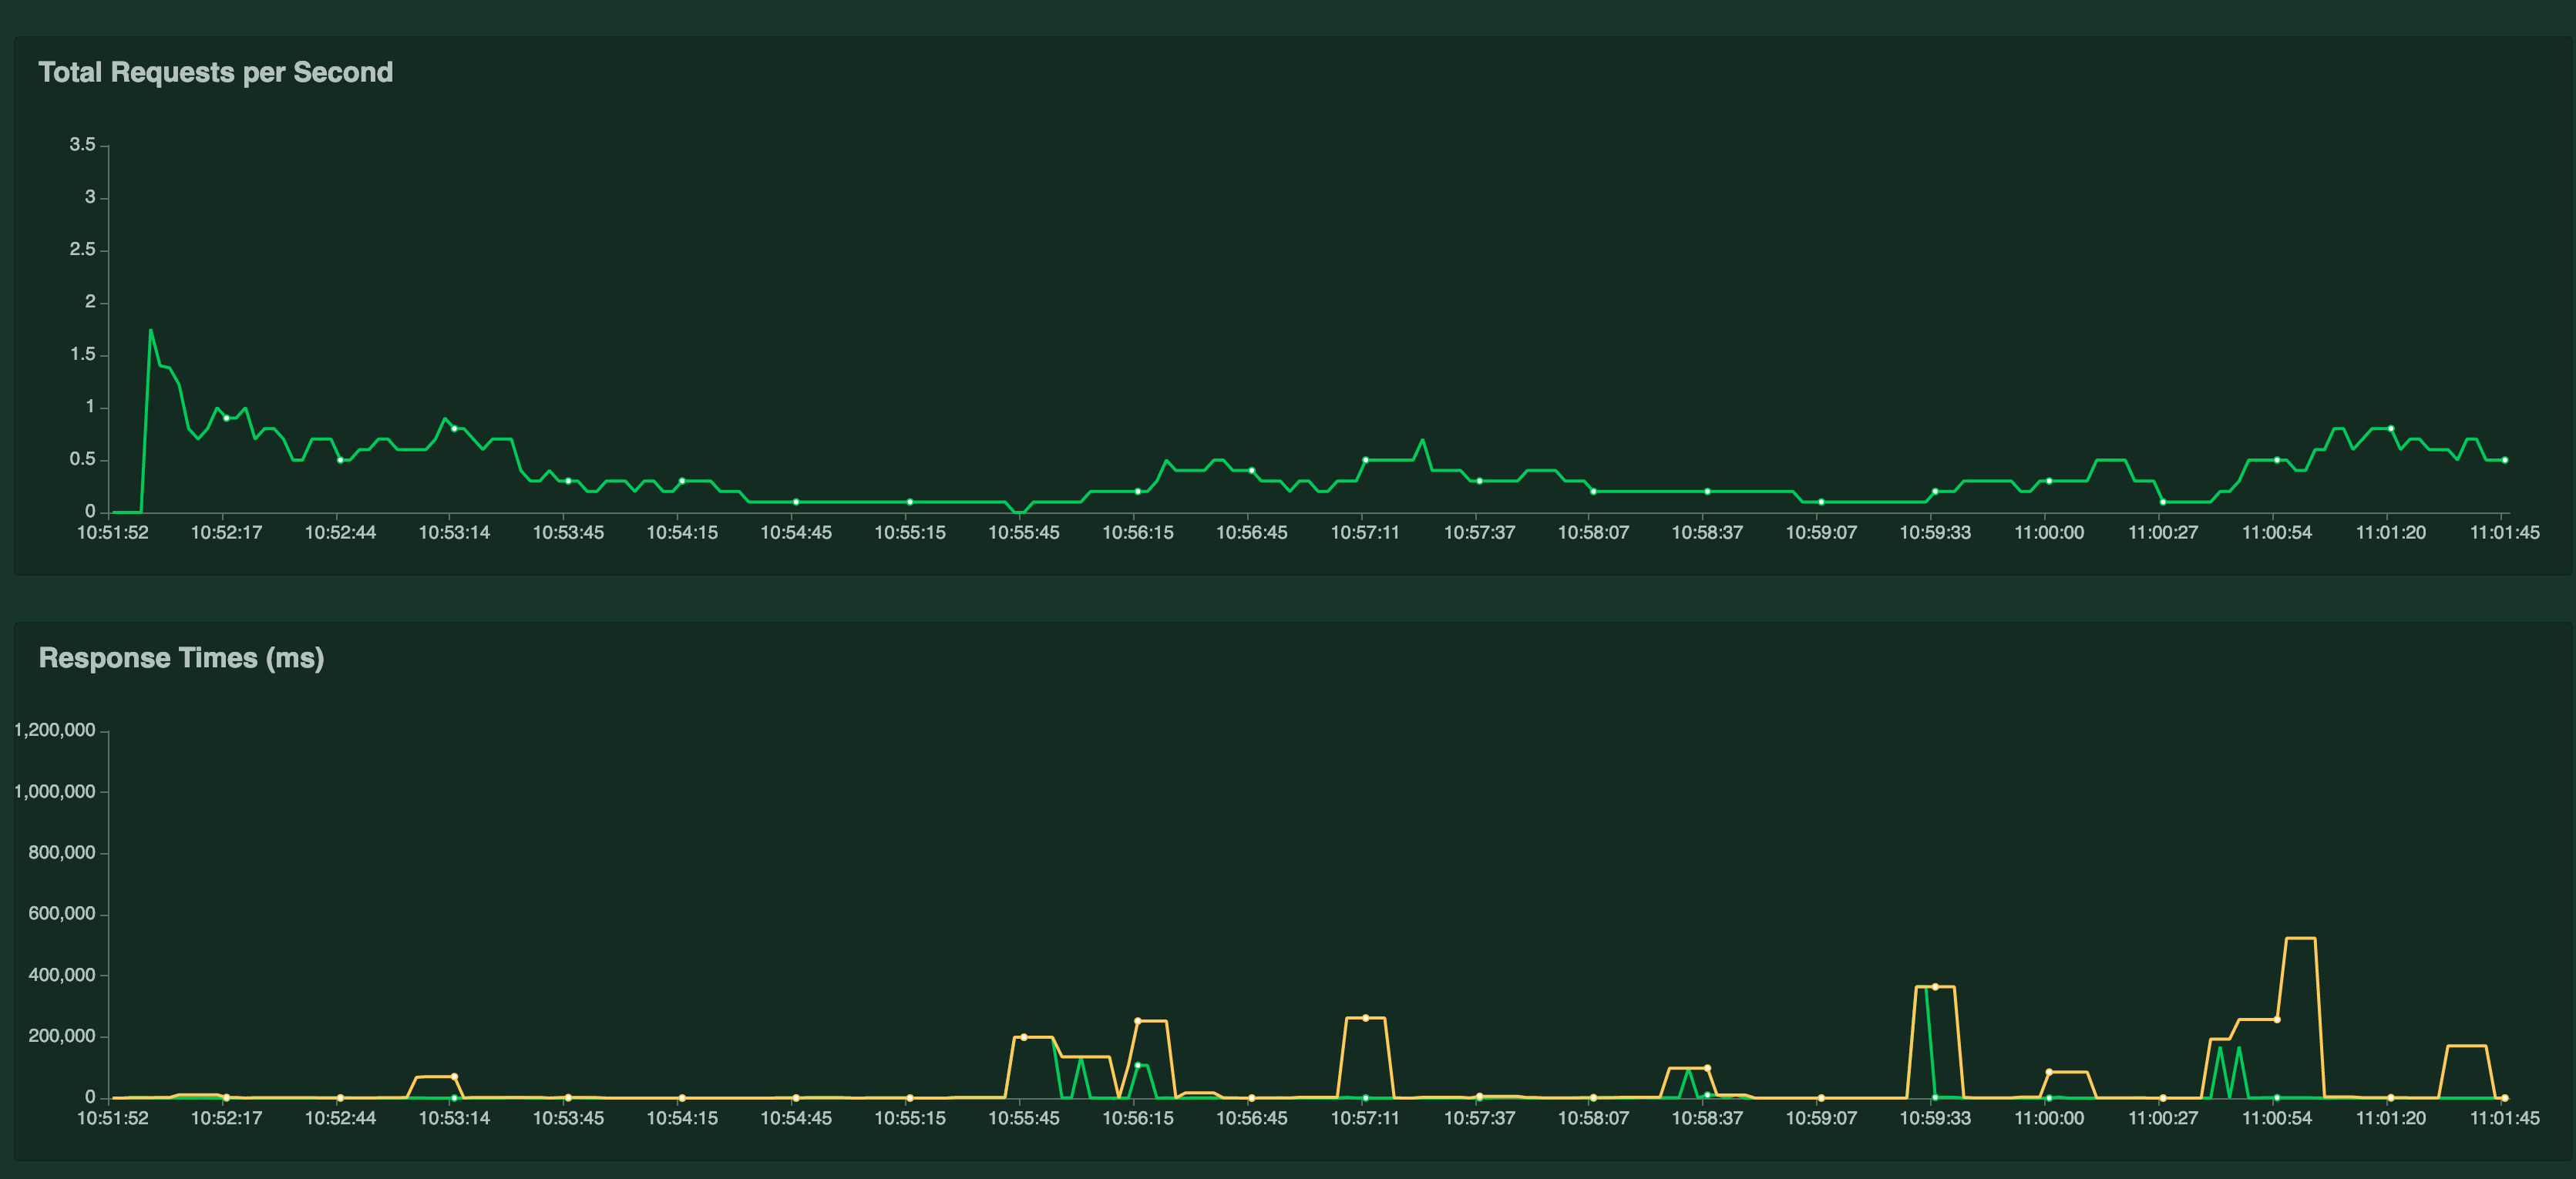
\includegraphics[width = 22cm]{./figures/10-users-original}\\[0.5cm] 
  \caption{Locust Statistics Dashboard for load of size 10 users}
  \label{fig:10-users-original}
\end{sidewaysfigure}

\begin{figure}[h!]
  \centering
  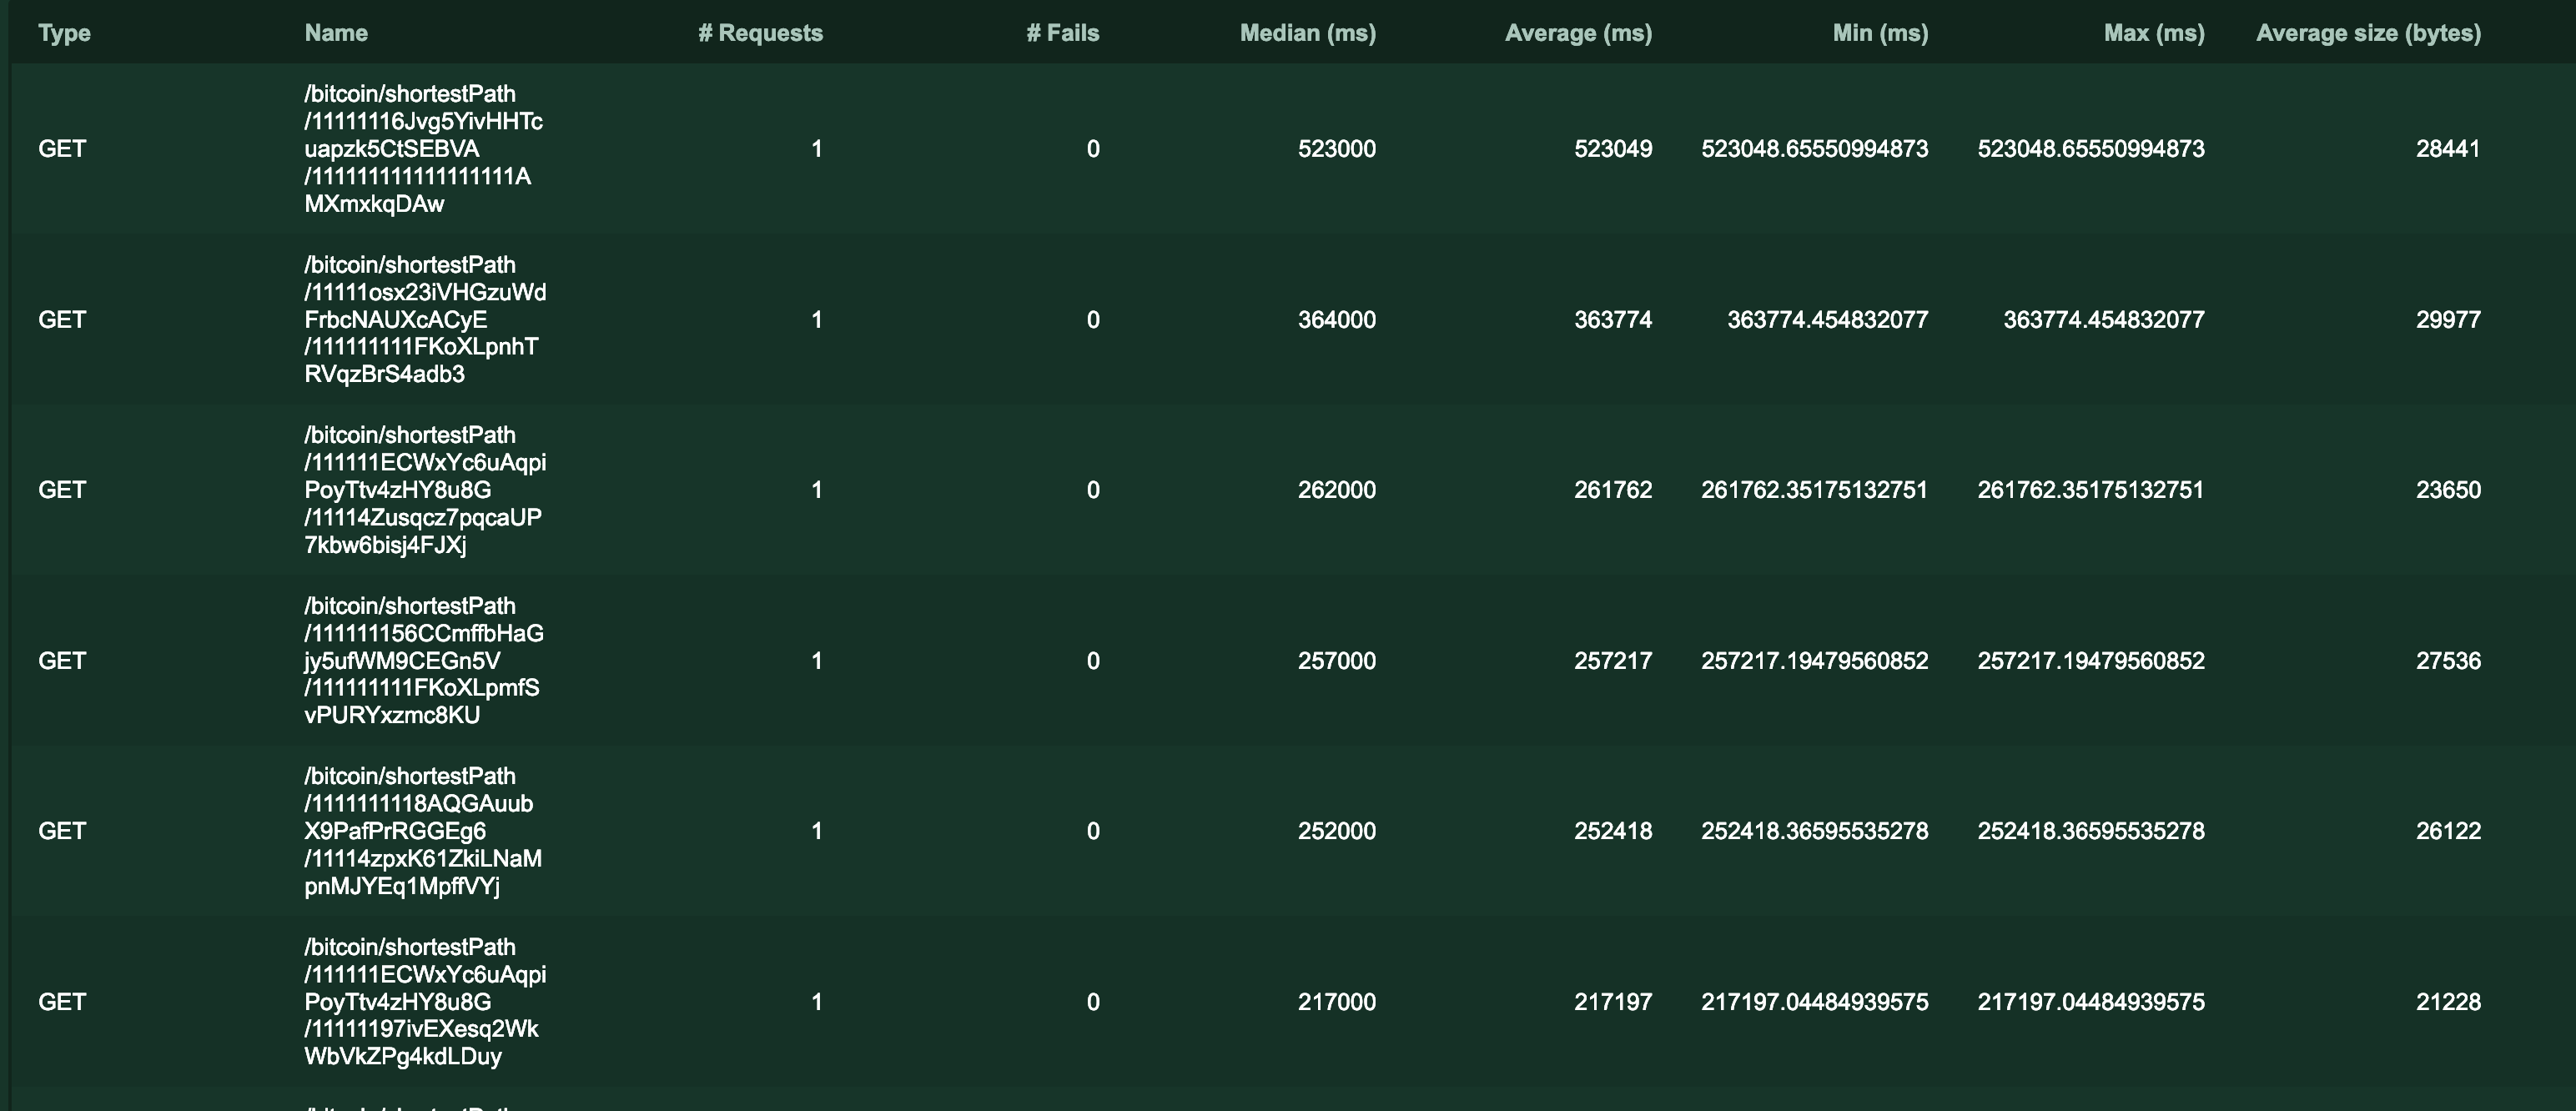
\includegraphics[width = 15cm]{./figures/10-users-original-culprit}\\[0.5cm]
  \caption{The Locust statistics dashboard for the requests ordered by decreasing response times; showing the shortest path requests to be responsible for response time spikes}
  \label{fig:10-users-original-culprit}
\end{figure}

\subsubsection{100 Concurrent Users}
I attempted this experiment in order to observe how the system behaves under a significantly larger load. The statistics dashboard for this experiment can be seen in \ref{fig:100-users-stats-dashboard}. 
\\\\
Observations:
\begin{itemize}
    \item At about one minute, there was a period where no responses were recieved (see the 'no data' label in figure \ref{fig:100-users-stats-dashboard}
    \item At this time, requests began to return errors of 500 series
    \item Investigation led us to discover the cause was due to the connection pool for the database becoming full and the timeout for waiting for a connection to become free had elapsed
    \item The connection pool became saturated due to several connections being consumed by expensive path finding tasks
    \item The significant latencies of the path finding tasks (for those that did return) can be seen in figure \ref{fig:100-users-path-finding-latencies}, and can be seen towards the end of the timeline in figure \ref{fig:100-users-stats-dashboard} where the response time spikes to the 150,000 ms (150 s) range. 
    
\end{itemize}

Clearly, invoking several concurrent path finding requests is problematic and will cause user requests (including non path finding requests) to fail. 
\begin{sidewaysfigure}[h!]
  \centering
  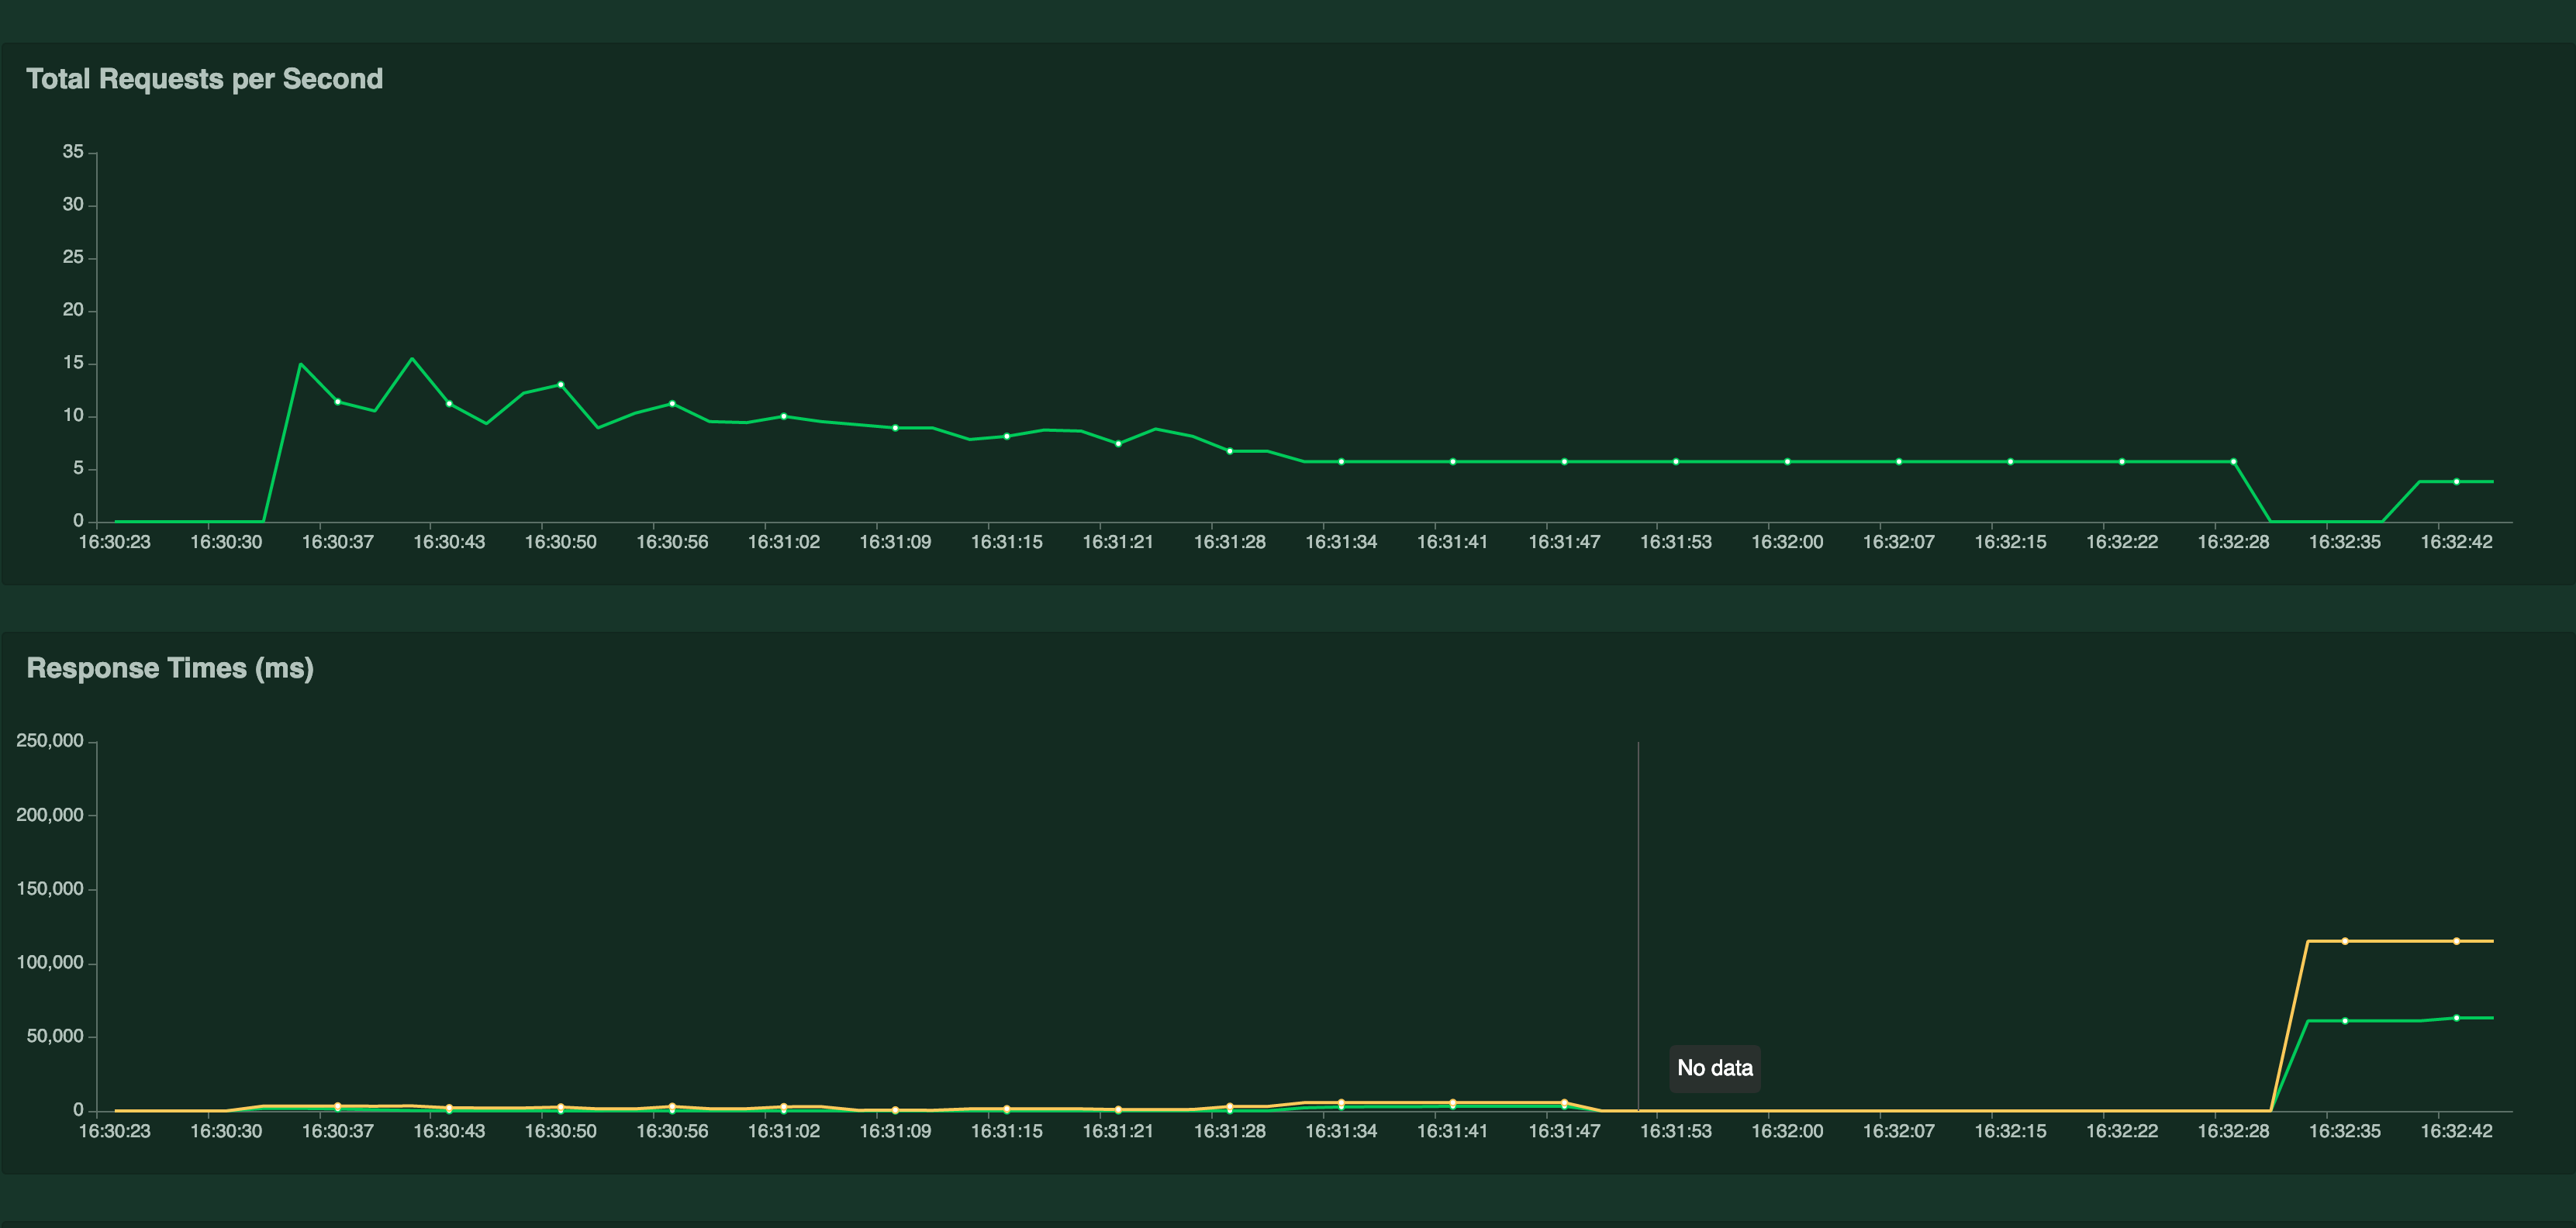
\includegraphics[width = 22cm]{./figures/100-users-performance-trace}\\[0.5cm] 
  \caption{Locust Statistics Dashboard for load of size 100 users}
  \label{fig:100-users-stats-dashboard}
\end{sidewaysfigure}

\begin{figure}[h!]
  \centering
  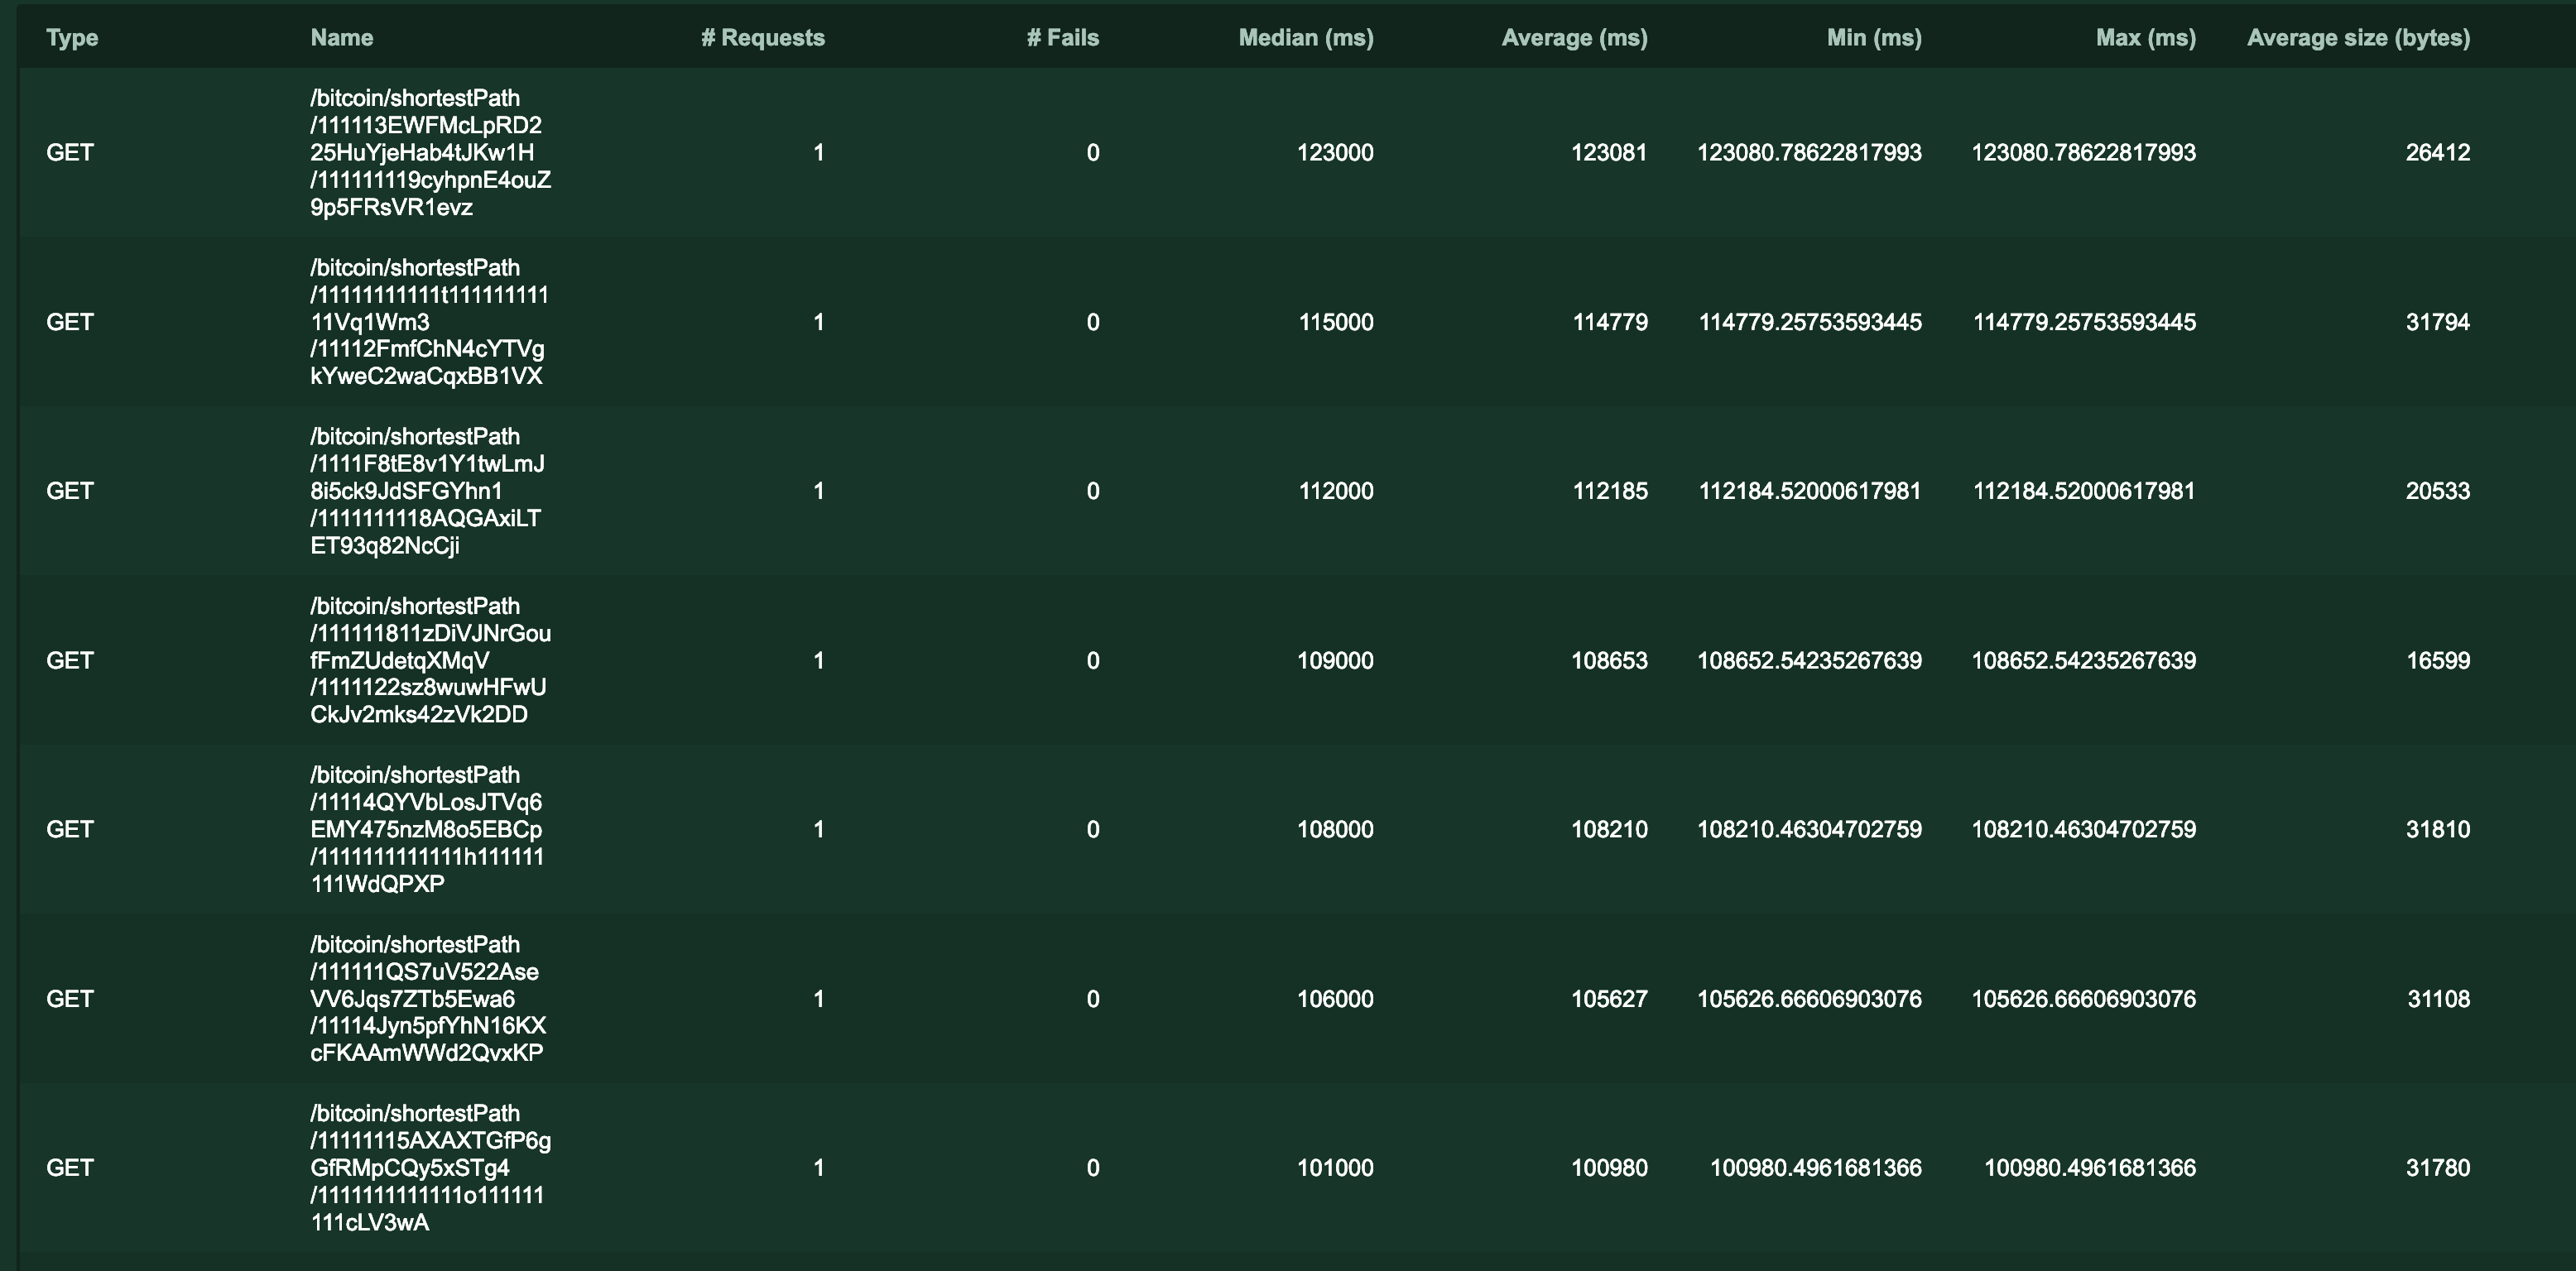
\includegraphics[width = 15cm]{./figures/100-users-shortestpath}\\[0.5cm]
  \caption{The Locust statistics dashboard for the requests ordered by decreasing response times; showing the shortest path requests to be responsible for response time spikes}
  \label{fig:100-users-path-finding-latencies}
\end{figure}

\subsubsection{10 Concurrent Users (no path finding)}
In order to observe how all other requests would behave without the path finding feature, we removed the path finding request from the users behaviour. 
\\\\
Observations:
\begin{itemize}
    \item A 0\% error rate
    \item There are still some spikes, that can be attributed to a few requests for Output entities [see figure \ref{fig:10-users-slow-outputs}]. 
\end{itemize}

\begin{sidewaysfigure}[h!]
  \centering
  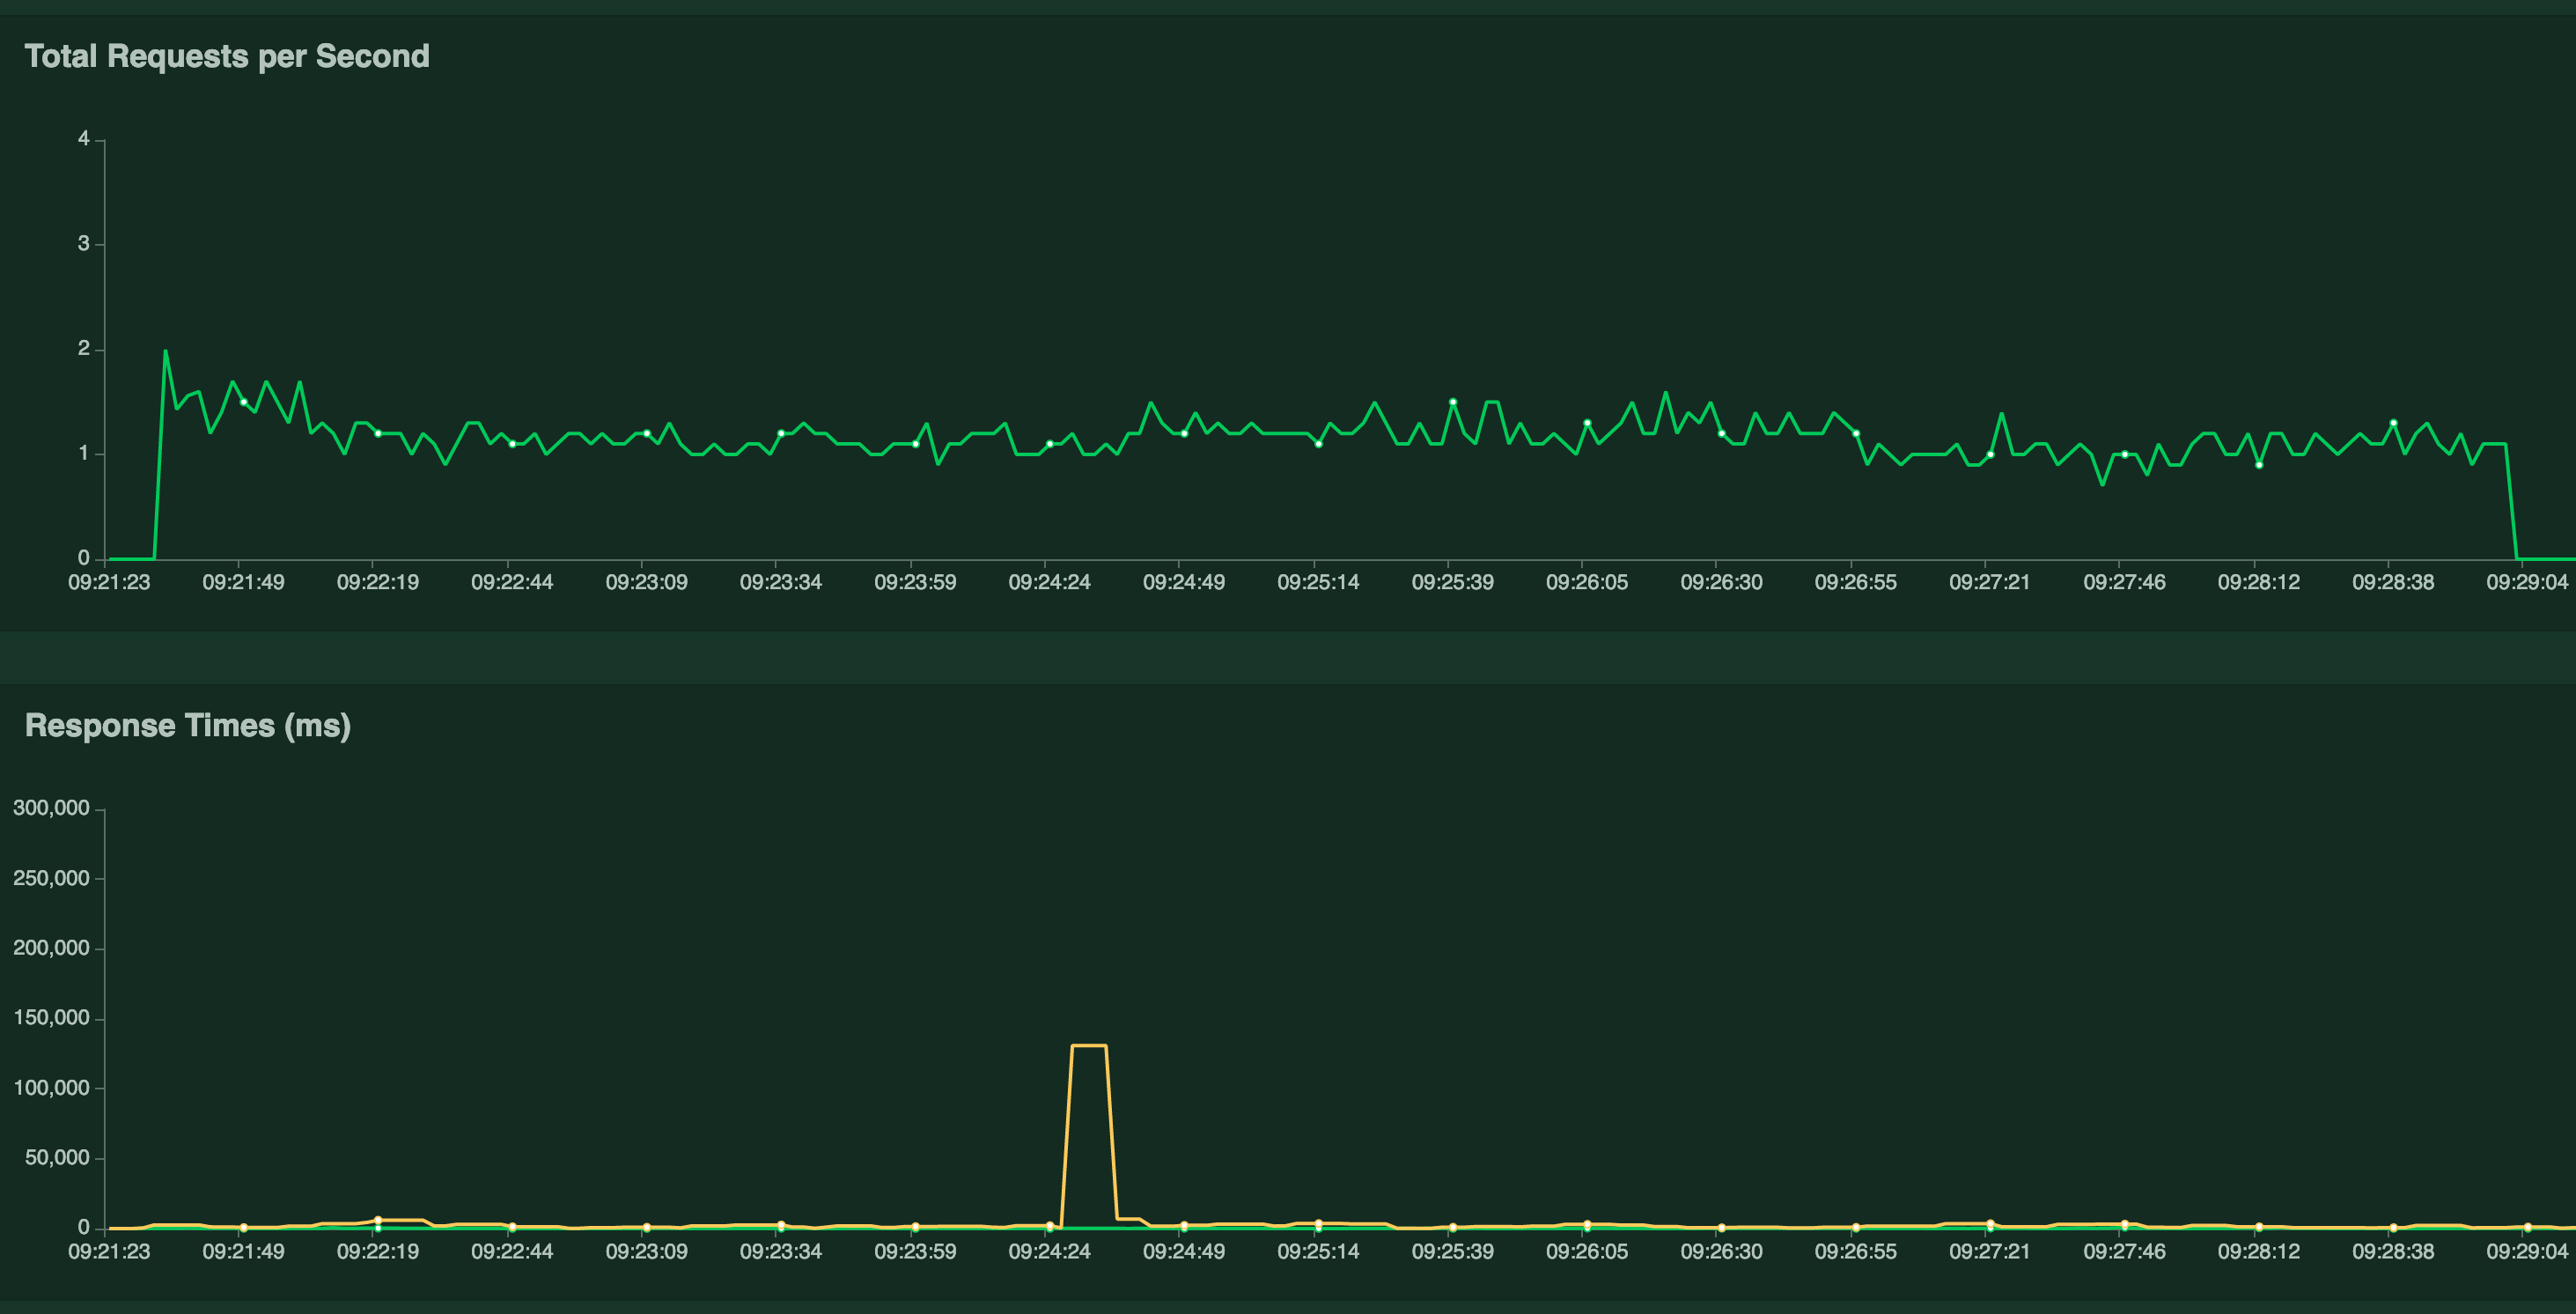
\includegraphics[width = 22cm]{./figures/10-users-no-path-locust}\\[0.5cm] 
  \caption{Locust statistics dashboard for load of size 10 users, without shortest path requests}
  \label{fig:10-users-stats-dashboard-no-path-finding}
\end{sidewaysfigure}

\begin{figure}[h!]
  \centering
  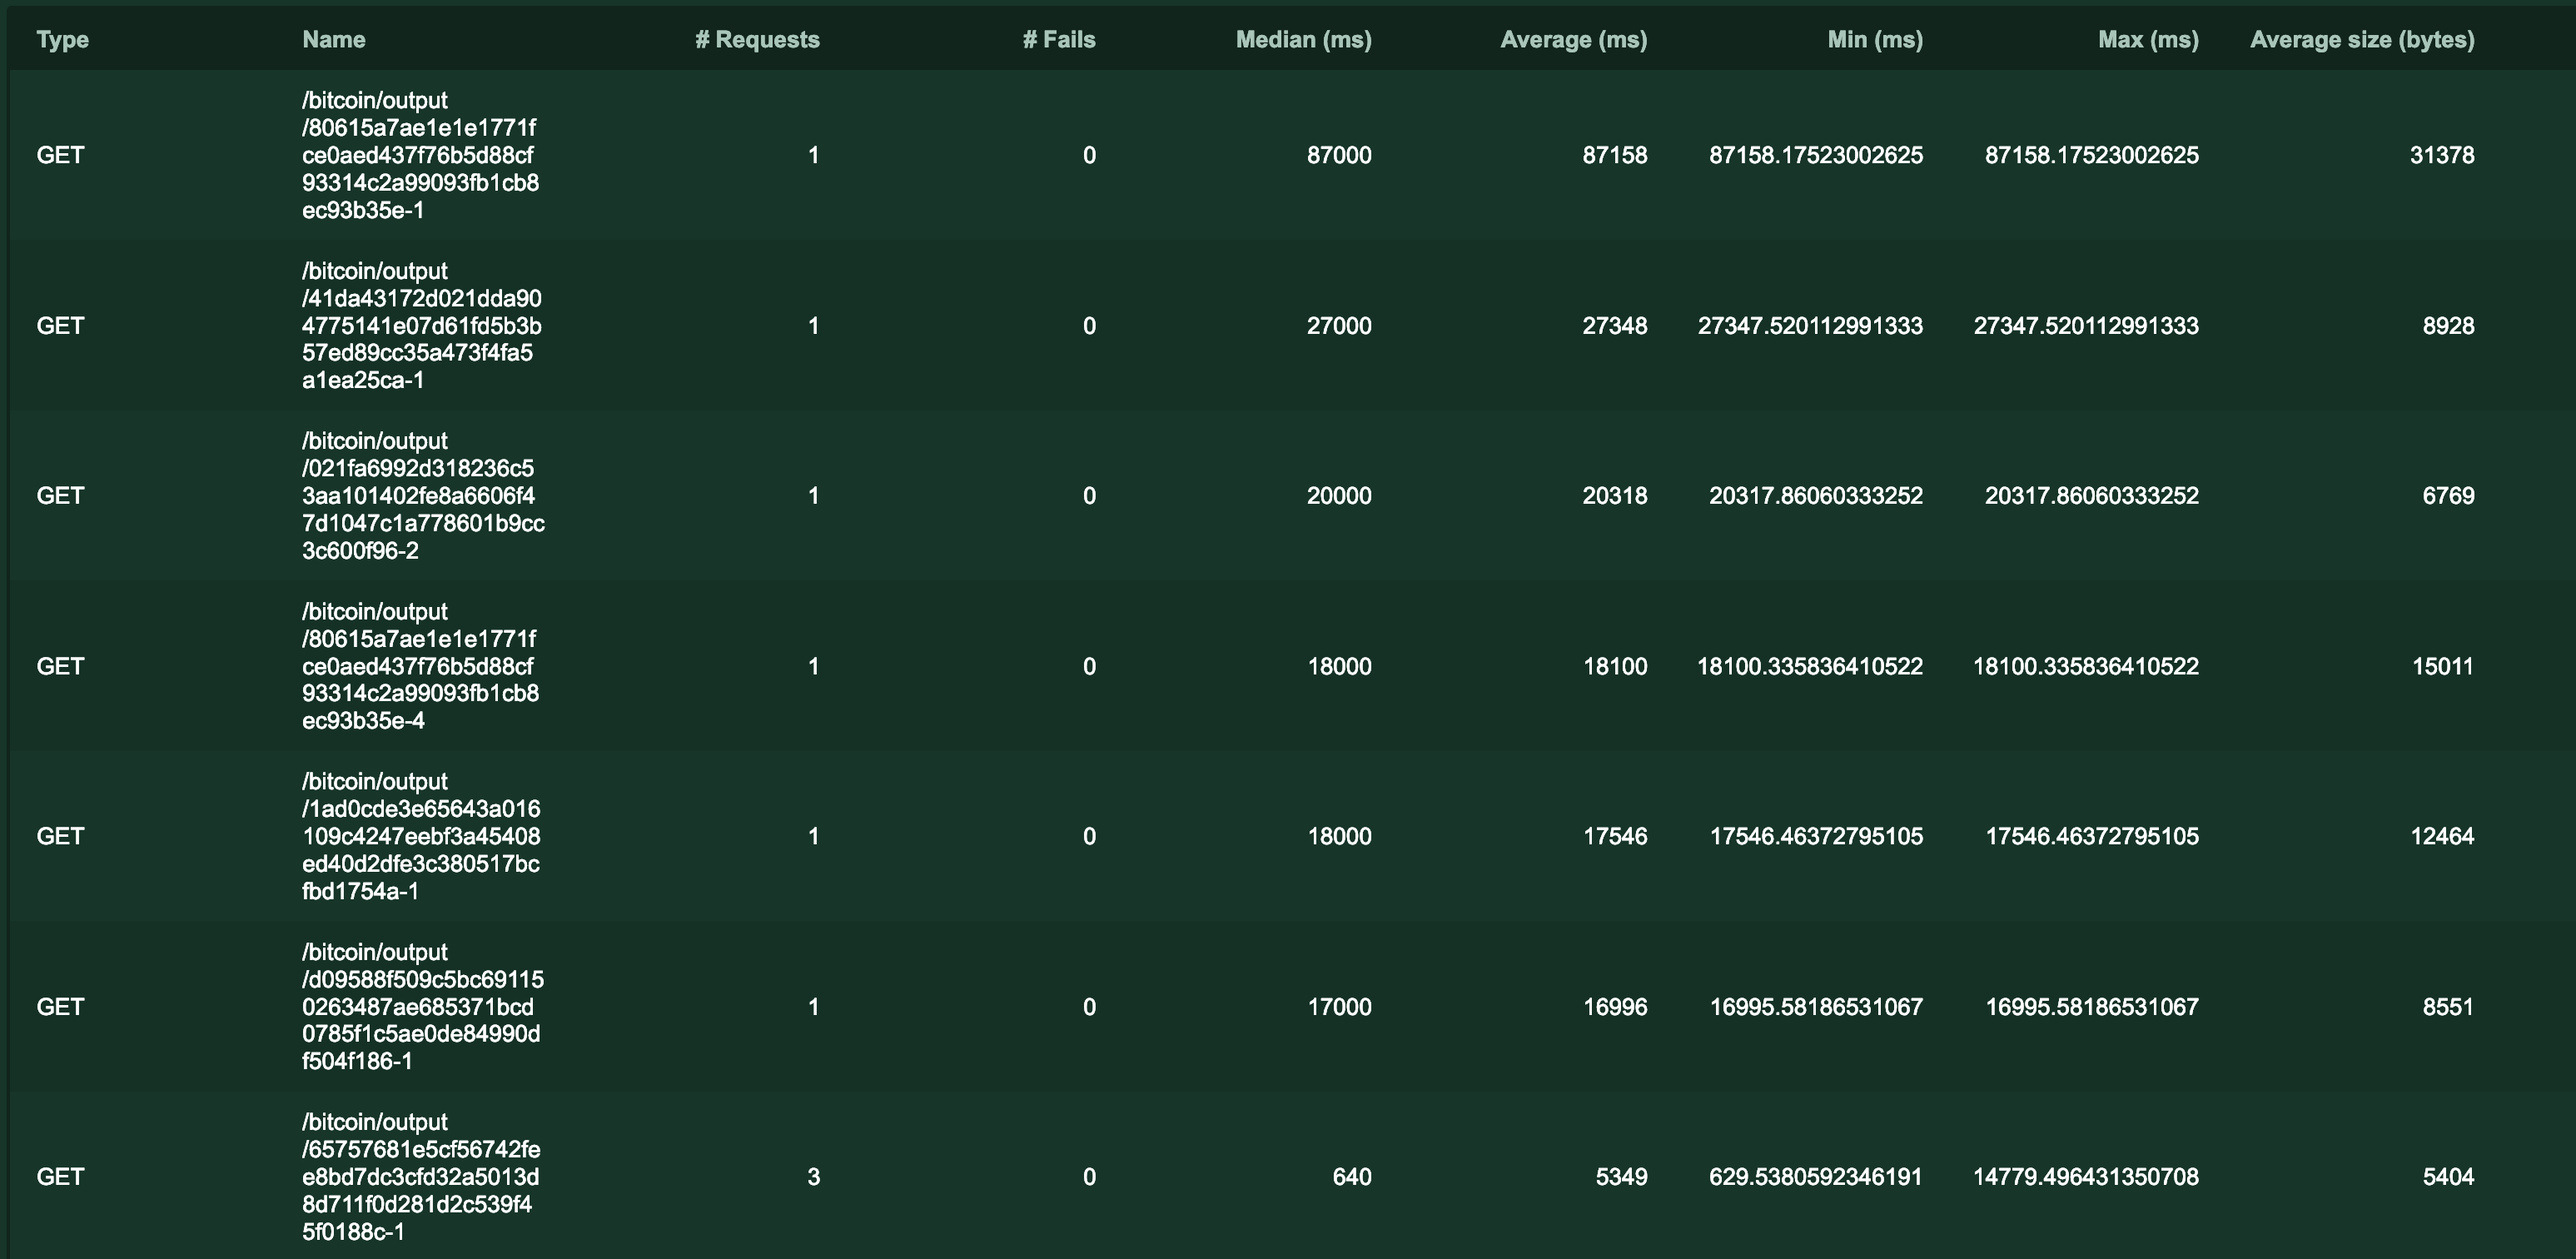
\includegraphics[width = 15cm]{./figures/10-users-no-path-culprit}\\[0.5cm]
  \caption{Locust statistics dashboard for load of size 10 users, showing requests ordered by decreasing response times; showing the output requests responsible for the spikes in figure \ref{fig:10-users-stats-dashboard-no-path-finding}}.
  \label{fig:10-users-slow-outputs}
\end{figure}

\subsubsection{10 Concurrent Users (no path finding + node limiting)}
Clearly fetching entities with an unbounded number of neighbours can cause issues, so we introduced the node limiting query parameter which is used to implement the 'node limiting' functionality as described
Observations:
\begin{itemize}
    \item 0\% error rate as before 
    \item Spikes now dampened due to node limiting
    \item Expected response rates for entire experiment 
\end{itemize}

\begin{figure}[h!]
  \centering
  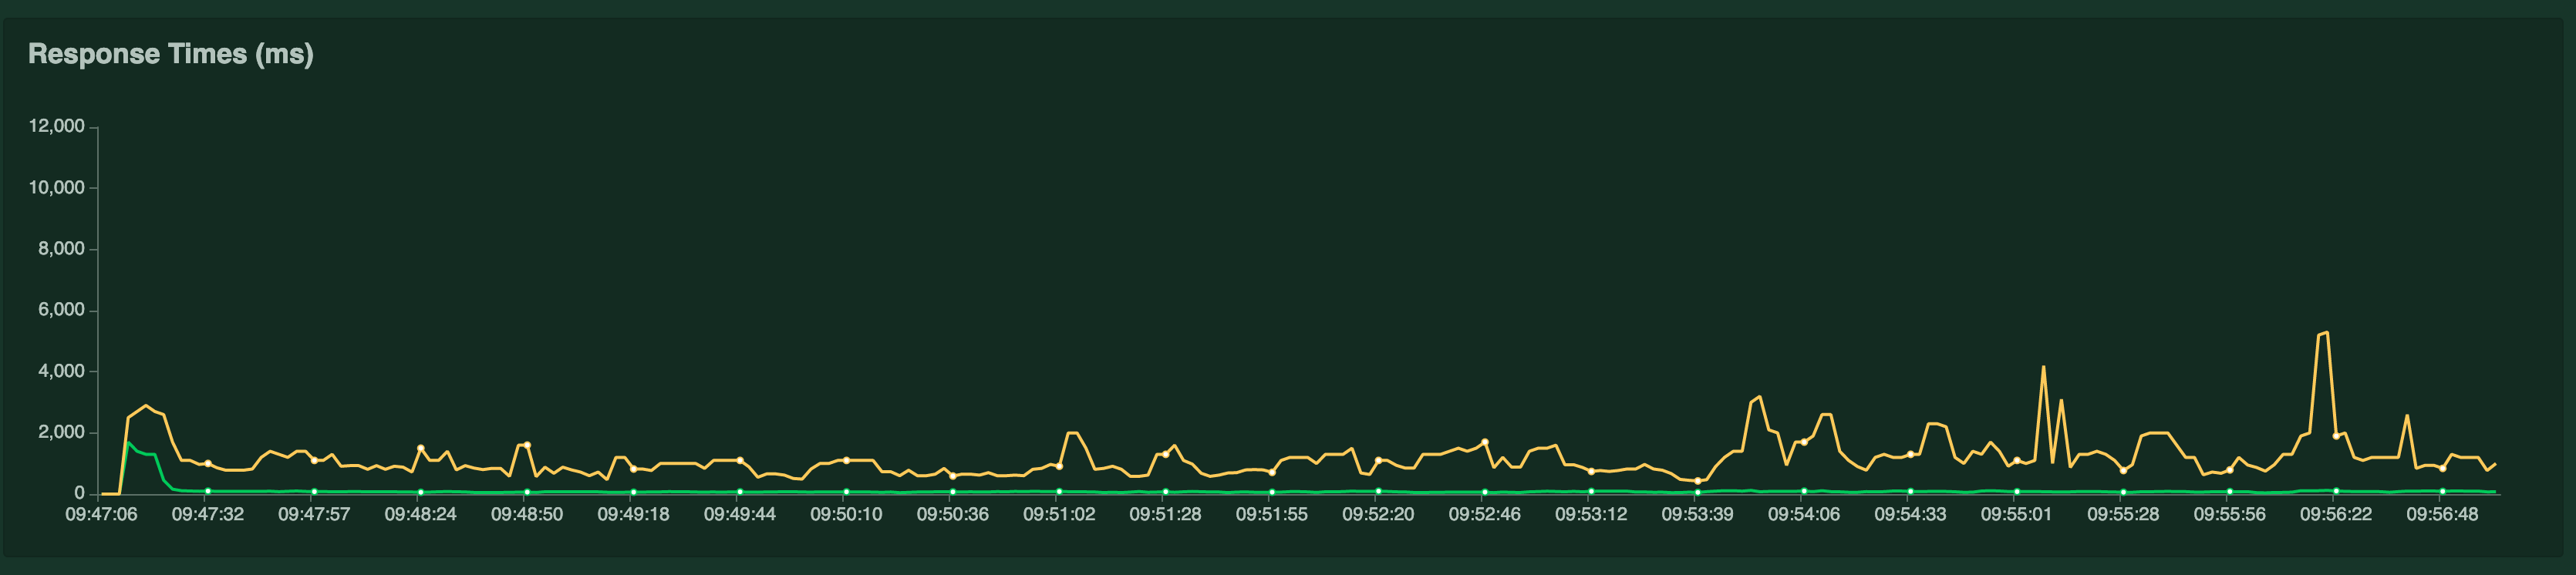
\includegraphics[width = 15cm]{./figures/10-users-no-path-with-limit}\\[0.5cm]
  \caption{Locust statistics dashboard for load of size 10 users, without path finding requests and including a node limit of 10.}.
  \label{fig:10-users-no-path-with-limit}
\end{figure}

\subsubsection{100 Concurrent Users (no path finding + node limiting)}
Observations:
\begin{itemize}
    \item Now a 0\% error rate due to absence of path finding request
    \item Spikes dampened by node limiting [see fig \ref{fig:100-users-no-path-with-limit}]
    \item Acceptable median response rates for entire experiment
    \item Slightly higher 95th percentile response times compared with 10 users, due to greater load
\end{itemize}

\begin{figure}[h!]
  \centering
  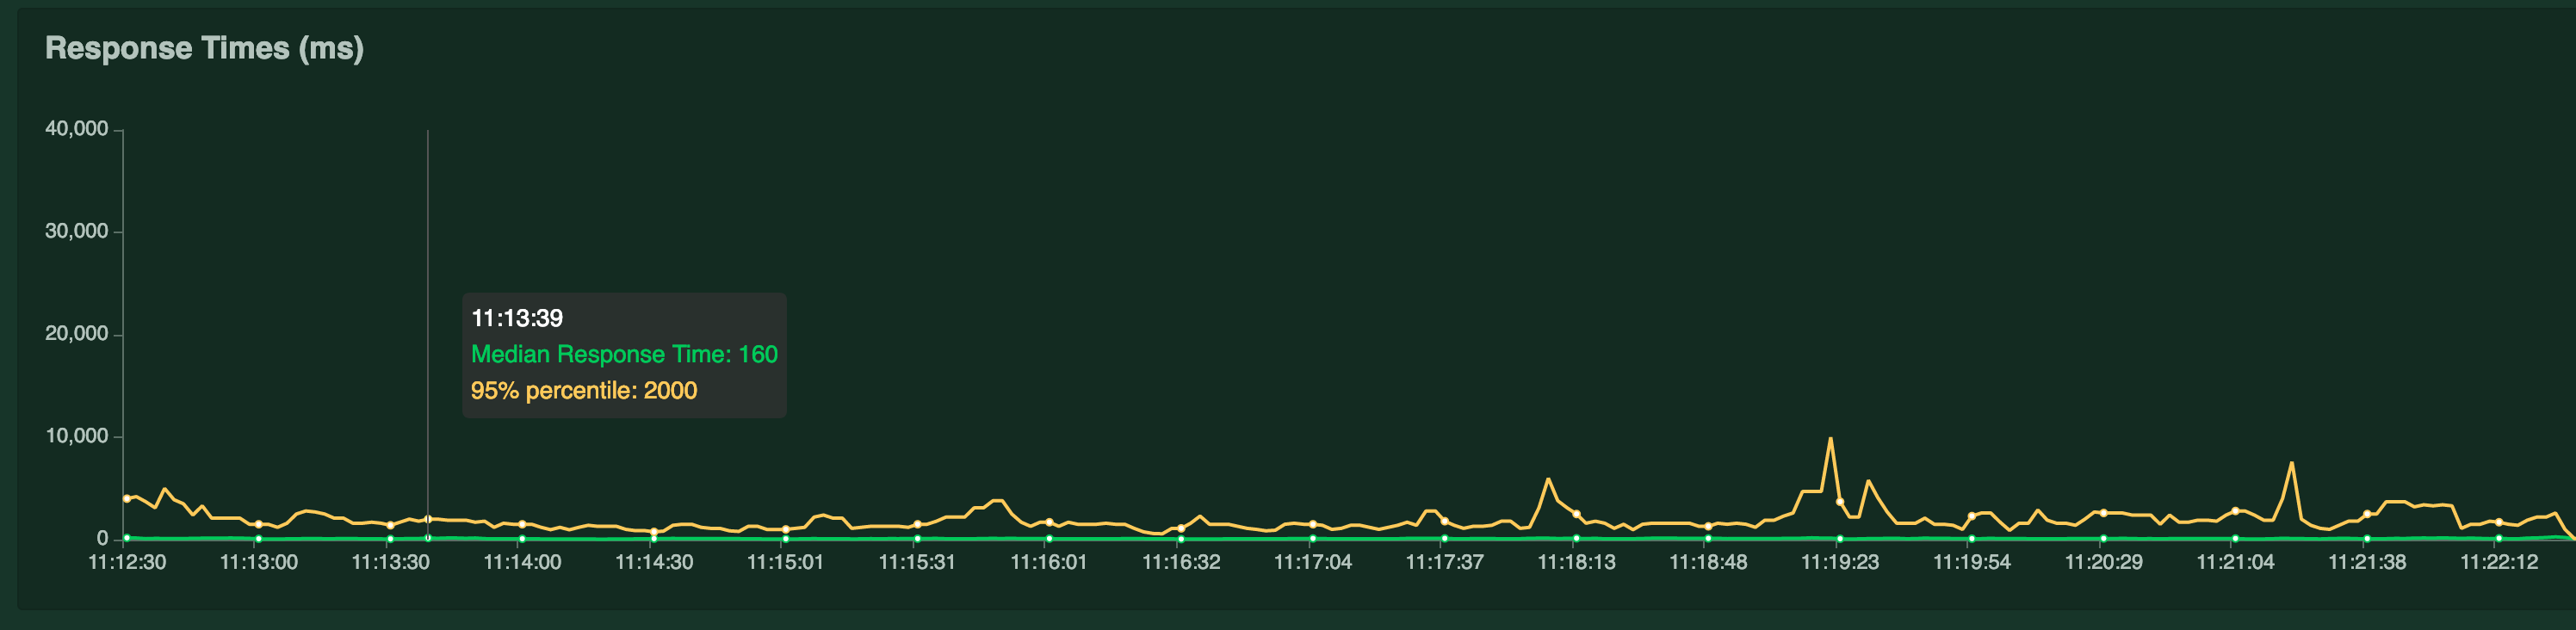
\includegraphics[width = 15cm]{./figures/100-users-no-path-node-limit}\\[0.5cm]
  \caption{Locust statistics dashboard for load of size 100 users, without path finding requests and including a node limit of 10.}.
  \label{fig:100-users-no-path-with-limit}
\end{figure}

\subsubsection{Conclusion}
From these experiments, I learnt that under significant load, the path finding queries are capable of causing a denial of service to other users of the system. Additionally, with requests that retrieve entities with an unbounded number of neighbours, request response times become less predictable. However, without path finding requests and with the default node limiting option enabled, the system will be able to handle considerable loads (up to 100 users) comfortably. 
\todo{import time too}

\subsection{Blockchain Import}
As described in section \ref{section-blockchain-import}, the import of the Bitcoin Blockchain up to block 570,000 took \textbf{5 hours, 32 minutes and 54 seconds}, which was performed in a VM with the specifications described earlier in section \ref{satoshi-specs}.
\\\\
The alternative approaches to performing this task are discussed in section \ref{design-db-previous-work}. These tools have the following performance metrics:
\begin{itemize}
    \item Bitcoin to Neo4J Tool : For block height 466,874, the GitHub page says it can take more than 60. Performed on Thinkpad X220 (8GB Ram, 4x2.60GHz CPU) \cite{RefWorks:doc:5c98e031e4b068320632cef2}. 
    \item TokenAnalyst Approach: Achieve the download and database population in a working day = ~9 hours. They took 6 hours to fetch all bitcoin data using RPC, then convert it to CSV format. TokenAnalyst explain how they had 32 cores at their disposal and were able to perform the import in 1 hour 10 minutes. 
    \cite{RefWorks:doc:5c98e0cde4b044512c0b8641}
    \item Blockchain2graph provides stress test information on their Github page which achieves 48,000 blocks in a 24 hour period.  \cite{RefWorks:doc:5cac6184e4b01c076c63e173}. They do not describe the hardware for this benchmark data; however their 'old' tests ran on an Intel Atom with 4GB RAM and 1 TB of disk space. 
\end{itemize}

\subsubsection{Existing solution comparison}
With such different hardware and block heights used for each of the above benchmarks, it would not be a useful to extrapolate the results above to the same block height or making very rough estimates on the performance improvements gained if equivalent hardware was used. Comparisons therefore need to be made both qualitatively and pragmatically. 
\\\\
Clearly, the performance of our approach far exceeds the implementation of the Bitcoin to Neo4J tool. The approach uses transnational queries to add data to the database which may explain the most significant performance issues with this approach. Neo4J's bulk import tool, used by our implementation, bypasses the transnational layer and is designed to heavily utilise parallelisation across multiple cores which vastly expediates this import process. 
\\\\
TokenAnalyst use the Neo4J import tool and are able to achieve a very impressive import time of over an hour; this is faster than our import time, but with the distinguishing factor of having many more cores than we had available, therefore allowing for greater parallelisaiton. This highlights that hardware is the bottleneck for our database population time. 
\\\\
Due to the relatively recent publication of TokenAnalysts article describing their process, we are able to assume their import process will be to a block height that was recent and therefore similar to the block height of 570,000 we used for the bulk import process.
\\\\
Comparing TokenAnalyst's download stage to our download stage, they are able to achieve writing the entire Bitcoin Blockchain data to CSV in 6 hours, compared to our 12 hours [see section \ref{section-blockchain-download}]. Again, greater physical resources will have given them greater ability to parallelise the workload and achieve better performance. However, one weakness in our approach is the necessity to manually intervene between sub-jobs (i.e between download of blocks 100k-200k and 201k-300k etc). This was done in order to mitigate the consequences of the overall job failed, however this mitigation could be replicated in an automated fashion in order to reduce idle time across the download period. 

\section{Performing a historical investigation}

want order by desc/asc with price
able to see incoming/outgoing easier - different colours
filter to show only incoming/outgoing 
Caching search params when navigating 
identify outputs to which addresses in supernode

The information I used to initiate the investigation:
* Theft date: 1st March 2012
* Exchange name: Bitcoinica 

I used walletexplorer.com to find the suitable wallet name for Bitcoinica for this date: this turned out to be Bitcoinica-old. I used this wallet name as a starting point of the investigation, only looking at transactions for the date 1st March 2012. 
\\\\
Initially, I searched for the wallet name with a date filter only. This rendered the view shown in figure \ref{fig:theft-no-filter}.

\begin{figure}[h!]
  \centering
  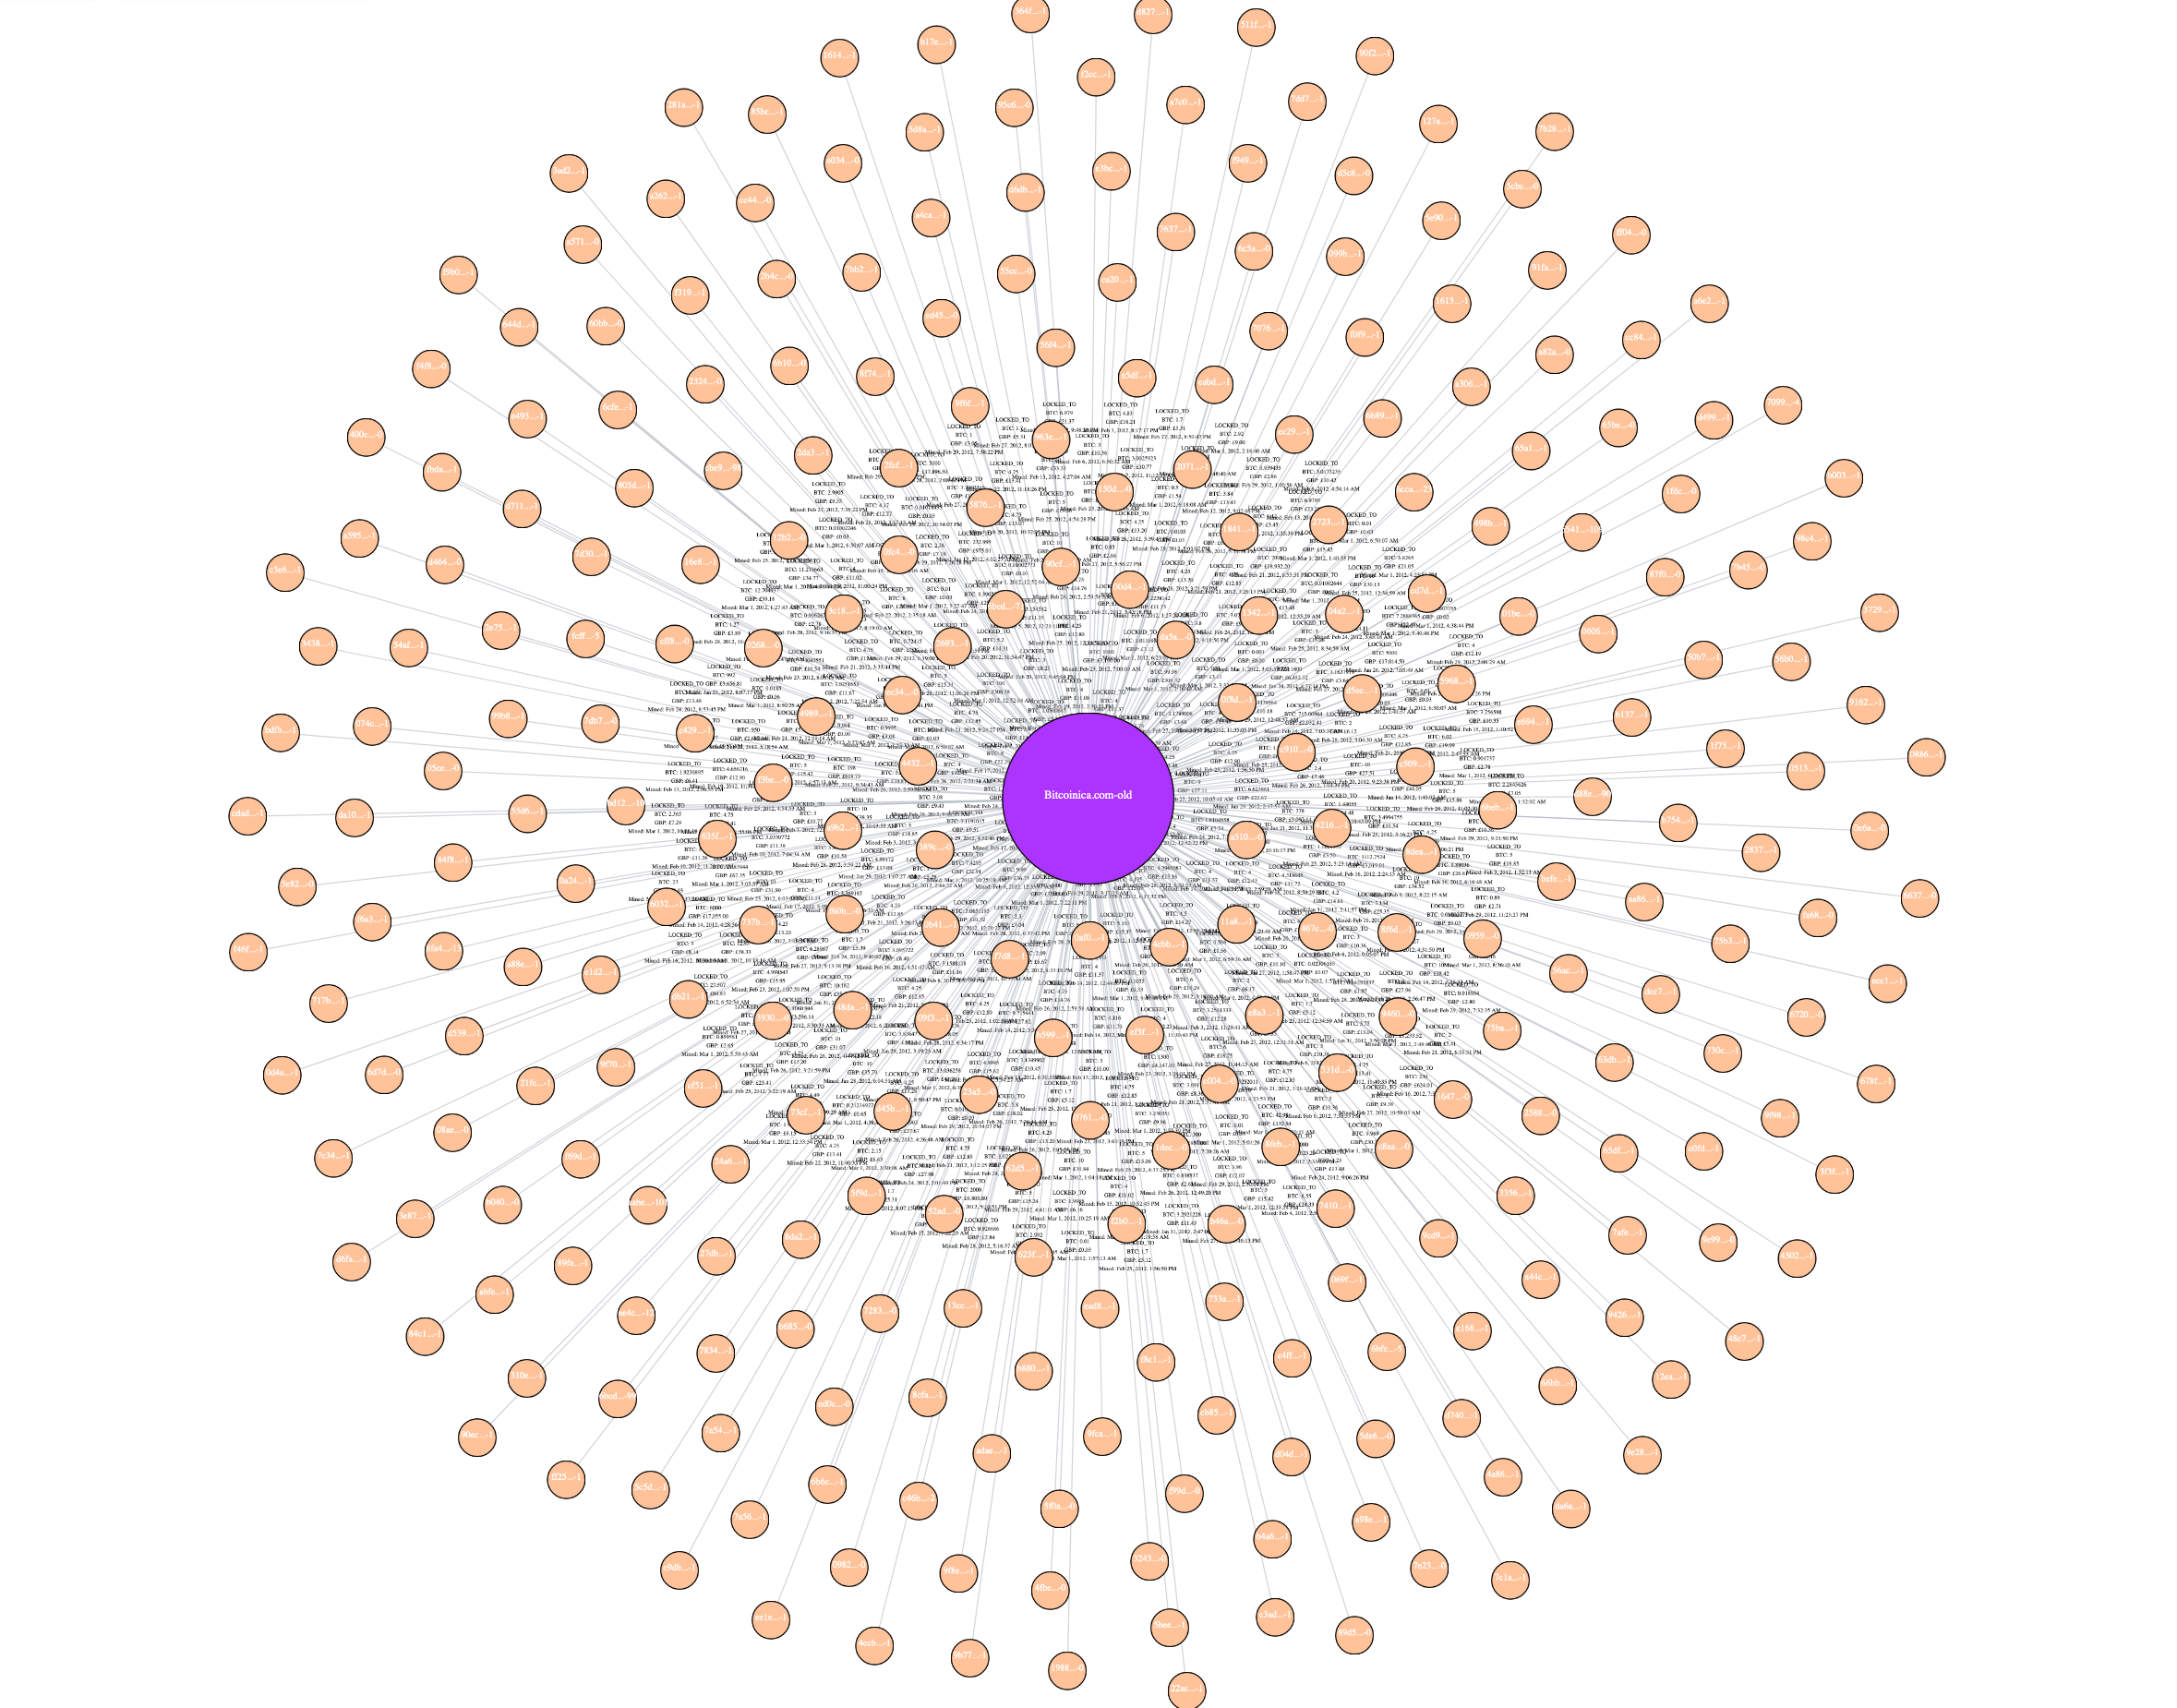
\includegraphics[width = 15cm]{./figures/theft-all-txs-1st-march}\\[0.5cm]
  \caption{A screenshot of the view when searching for entity Bitcoinica.com, filtered by date on 1st March 2012 only}.
  \label{fig:theft-no-filter}
\end{figure}

Obviously the huge amount of information shown in figure \ref{fig:theft-no-filter} is not feasible to digest and understand; therfore I navigated back to the search form to start refining my filters to help better specify what I am looking for. 
\\\\
I first added price filters in order to show only the high value transactions on the 1st of March; I filtered transactions to only show outputs that were spent of value more than $1000BTC$. 
\\\\
I then proceeded to inspect the outputs that were spent on the 1st of March that were of the greatest value [see fig \ref{fig:theft-highest-value-outputs}]. By doing so, and expanding out several other high value outputs spent on that day, I was able to identify transactions that spent a large amount of funds. I considered these transactions as suspicious.
\\\\
The suspicious transactions I identified through this process due to the size of funds they spent on this day were:
\begin{itemize}
\item \texttt{7b45c1742ca9f544cccd92d319ef8a5e19b7dcb8742990724c6a9c2f569ae732}: This transaction in total spent \textbf{20,555.1 BTC} - sending all \textbf{20,555 BTC} to one address and \textbf{0.01 BTC} to another. Using the neighbour expansion feature, I traced the bulk of the funds: 
20555BTC to 1DMuVKe9PKpx3dbs2b2MnXuVmLfA4drHif
25000BTC to 128u4nNS2DCbPk61aNAXLUTsHZt5FAEtit
24900BTC to 18E4d3JtQNyUBdxQ4y8ck6RUKXEb7W4KA7
23900BTRC to 1D56cDkVmoNGw7YmewL5boFwHyzEgDpygE
23399BTC to 1LJn39nzrwqM8MkevfSDCa1uVZCgJSTMtq
22399BTC to 13Fd5f8yFZCAAbtKQiNcWUmdbUNpVpznA6
21899BTC 1HZHp77ftbAEy4PQc8wuAahvPnpZHKMfmc
16899BTC 1Czhv7mDRNPMrzU9Ja7QkYSAvforGKQ2mv + 500BTC to 1Q3bsvTBcWF32Bt8FZgKAx7s43crvN9RVi (did not spend same day until July 31st 2012)
16900 to 1Q3bsvTBcWF32Bt8FZgKAx7s43crvN9RVi (spent next day on second of march)
17000 to 1BKF8kXHsNdQk6f5FognK4ZJCCBifE8ugm
15476 to 1MXe7zFRHx9KMwGKAGi2GvTbsHFDgVjcEw
12544 to 15GPUomoHVJbBsgY6eWdsKKaV3dywL5poj
12044 to 12F1GhUbVJvNW6ki1fRG1ZgeTkm2FixLLi


[9264 to 14Qr38dfmXZJUuxYaJxaTjg7yYcj5GDTqy - supernode cluster which 1BKF8kXHsNdQk6f5FognK4ZJCCBifE8ugm with earlier 17000 was paid to]

Supernodes then collect funds in tx, sends 9751 to 18ywk3t8XFtkEqMJt8hPG14D3gzTshB4YW

Does not spend funds till 4th August 2012
This seems to be the begining of another chain, spending sums of 100-1000 BTC (usually round numbers such as 100m 200, 500 etc) in each transaction, each transaction having only two outputs until the main large funds reduce down to just over 1000BTC with transaction fbab826df674b1e2ae3bedfc566f2692b8940ac1058605fe549753b34ebd8f0d. This seems to be the end of the peeling chain, as transactions now have several inputs and smaller outputs arent round numbers, more common to normal spending, therefore and loook lesss characteristic of a peeling chain. 


At this point, I wished to continue the investigation by following the address 1Q3bsvTBcWF32Bt8FZgKAx7s43crvN9RVi into the next day. 

\item \texttt{0268b7285b95444808753969099f7ae43fb4193d442e3e0deebb10e2bb1764d0}


This was a sum of 10000 BTC sent to address 1AaXeH5DuP6FpPxdCn9RGXKWhSG4r9Hq9q. Not spent until March 27th 2012.


\item \texttt{a82ad85286c68f37a2feda1f5e8a4efa9db1e642b4ef53cb9fd86170169e5e68}
\item \texttt{a57132e2cbc580ac262aa3f7bac1e441d6573f9633118bc48009618585a0967e}
\item \texttt{901dbcef30a541b8b55fae8f7ad9917ef0754bda5b643705f3773e590785c4d3}
\item 

\end{itemize}

\begin{figure}[h!]
  \centering
  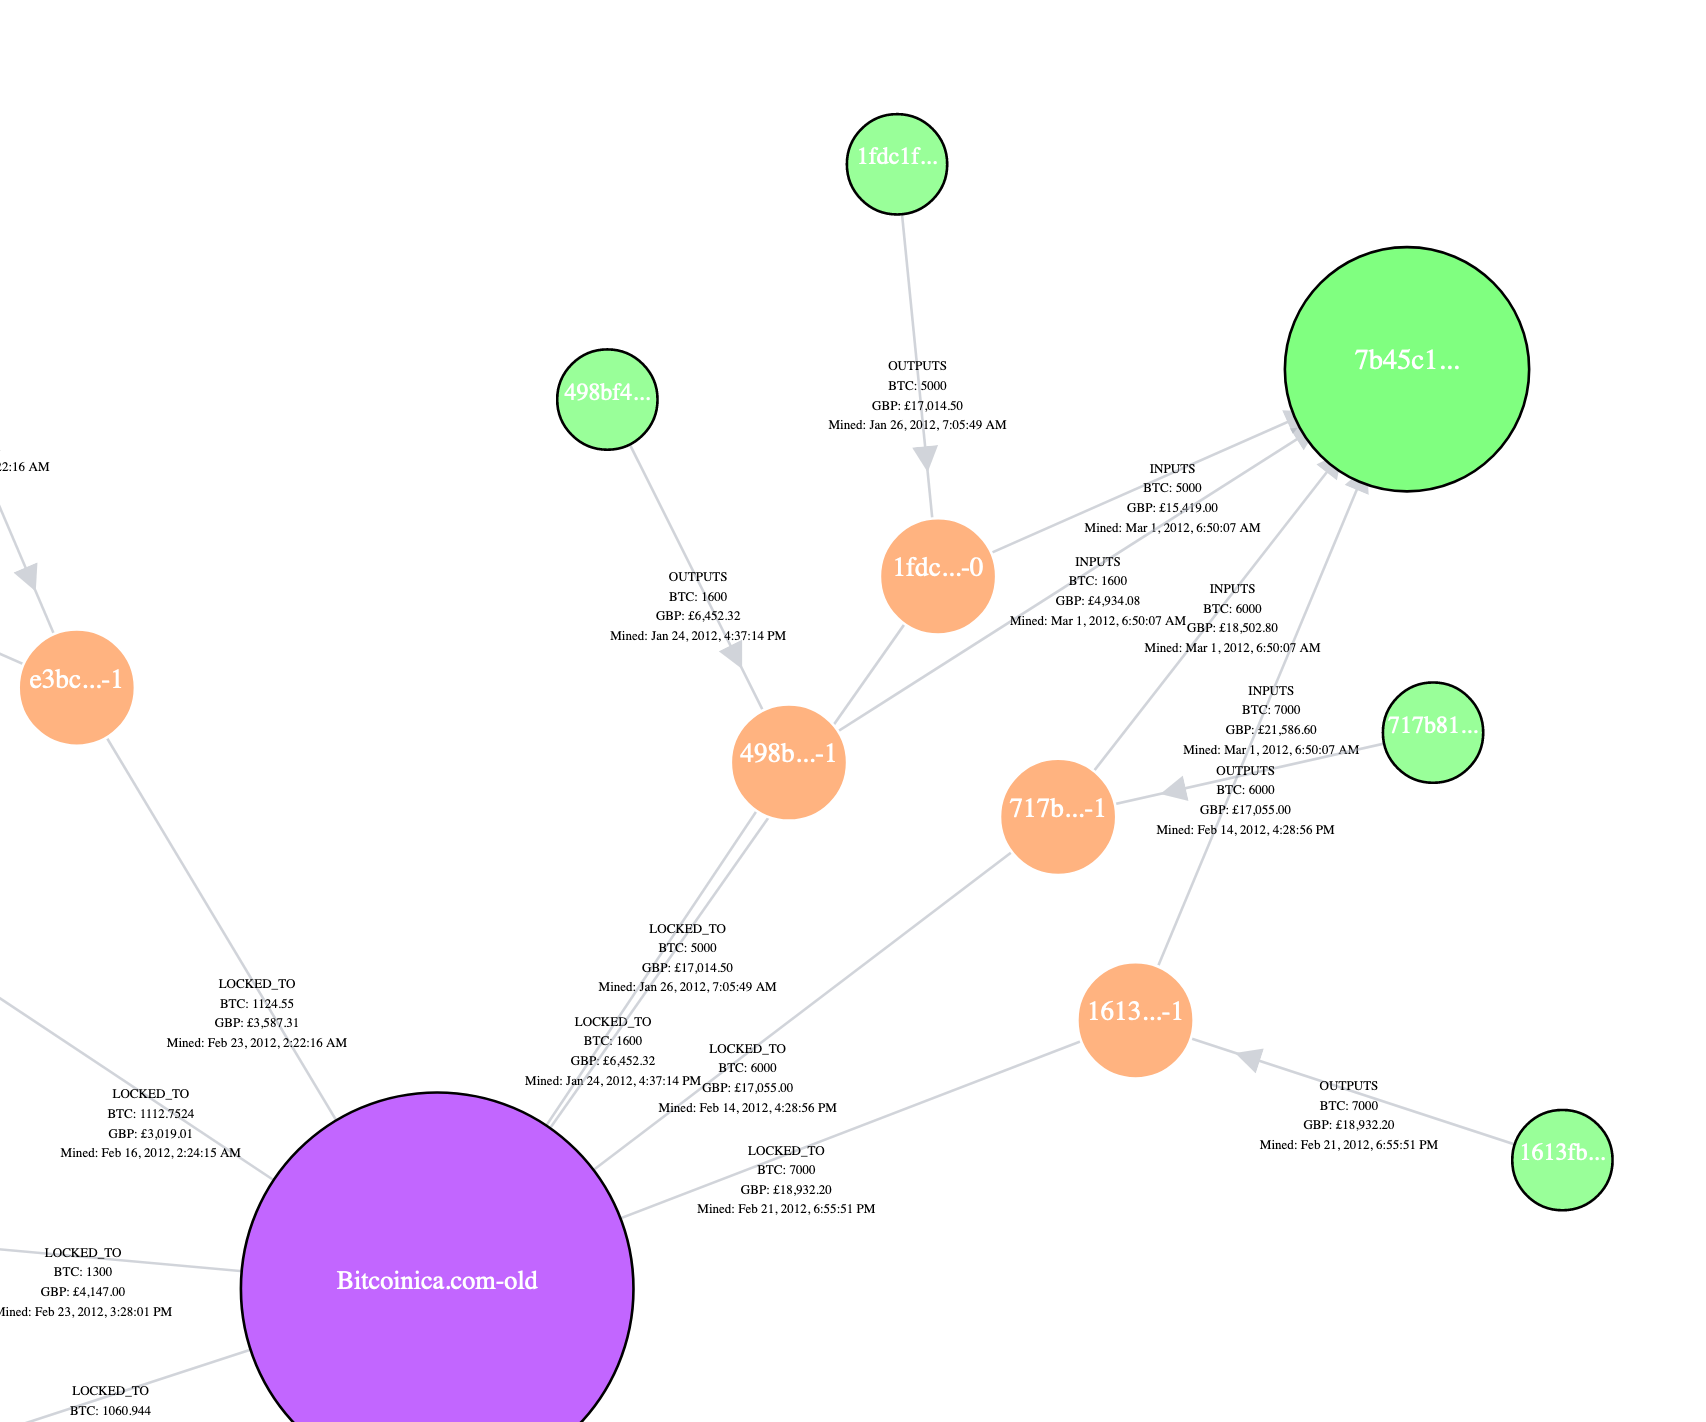
\includegraphics[width = 15cm]{./figures/theft-high-value-tx}\\[0.5cm]
  \caption{A screenshot of the view when searching for entity Bitcoinica.com, filtered by date on 1st March 2012 and by price, showing outputs spent with value > 1000BTC. Showing specifically the transaction spending the highest value outputs}.
  \label{fig:theft-highest-value-outputs}
\end{figure}